\documentclass[11pt]{article}

\usepackage[margin=1.5in]{geometry}
\usepackage{graphicx}
\usepackage{amsmath,amssymb}
\usepackage[hyphens]{url}
\usepackage[colorlinks=true,
            linkcolor=blue!60!black,
            citecolor=blue!60!black,
            urlcolor=blue!60!black]{hyperref}
\usepackage{booktabs}
\usepackage{enumitem}
\usepackage{xcolor}
\usepackage{tikz}
\usetikzlibrary{arrows.meta,positioning,shapes.geometric,fit,calc}
\usepackage{listings}
\usepackage{fancyhdr}
\usepackage{colortbl}
\setlength{\emergencystretch}{3em}
\newcommand{\mapsec}[3]{%
  \smallskip\noindent
  \begin{tabular}{@{}p{3.2cm}p{9.8cm}@{}}
  \toprule
  \textbf{Tasks / sources}    & #1 \\
  \textbf{Research questions} & #2 \\
  \textbf{Threats addressed}  & #3 \\
  \bottomrule
  \end{tabular}\smallskip}


\lstset{
  basicstyle=\ttfamily\small,
  keywordstyle=\color{blue!70!black},
  commentstyle=\color{green!50!black},
  stringstyle=\color{red!60!black},
  frame=single,
  breaklines=true,
  numbers=left,
  numberstyle=\tiny\color{gray},
  xleftmargin=2em
}

\pagestyle{fancy}
\fancyhf{}
\rhead{\small S2-D2 Proposal --- DRAFT}
\lhead{\small Tamper Detection and Data Integrity}
\cfoot{\thepage}

\title{%
  \textbf{Tamper Detection and Data Integrity for Self-Describing Scientific Data}\\[0.5em]
  \large A Research Plan for the S2-D2 Framework\\
  Using ClawHDF5 as an Experimental Platform
}

\author{
  M.~Scot Breitenfeld\\
  The HDF Group\\
  \texttt{brtnfld@hdfgroup.org}
}

\date{Draft --- \today}

\begin{document}

\maketitle

\begin{abstract}
This document proposes a research plan within the S2-D2
(Securing Self-Describing Data) project that addresses the Task~3
(data authentication) objective for HDF5, informed by the HDF5
SHINES (Securing HDF5 for Industry, National Security, Engineering,
and Science) security taxonomy developed under the NSF Safe-OSE
program~\cite{shines}. The proposal first surveys the state of the art in
tamper detection and data-integrity primitives---error-detection codes,
cryptographic hashes, message authentication codes and authenticated
encryption, classical and post-quantum signatures, hash trees and
authenticated data structures, cryptographic accumulators, polynomial and
vector commitments, transparency logs, trusted hardware attestation,
filesystem and cloud-store integrity mechanisms, and existing scientific-format
checksums---and derives a set of requirements (sub-dataset partial verification,
tamper localization, in-place and incremental update support, verifiable subset
extraction, public verifiability, no trusted setup, post-quantum upgradeability,
and HPC-feasible build cost). From this comparative analysis we conclude that
a Merkle-tree provenance scheme is the only primitive that simultaneously
satisfies all of these requirements \emph{without a trusted-setup ceremony and
without a pairing- or factoring-based primitive that Shor's algorithm breaks},
and we then design,
implement, and evaluate such a scheme in ClawHDF5~\cite{clawhdf5}. Beyond
the systems architecture (hybrid root-attribute plus chunked companion
dataset, Encrypt-then-MAC filter-pipeline ordering, version-counter nonce
derivation for safe in-place updates), the work targets three publishable
research contributions: (i)~a \emph{verifiable subset extraction} protocol
enabling a recipient of an arbitrary hyperslab to cryptographically verify it
as a true subset of a signed parent dataset; (ii)~a \emph{post-quantum hybrid
signing} scheme (Ed25519~$+$~ML-DSA-65) measured at HDF5 scale, addressing the
50-year archival timescales typical of scientific data; and (iii)~a
\emph{symbolic security analysis} (Tamarin or game-based) of the
EtM~$+$~version-counter~$+$~signed-root construction, evaluated against a
white-box adversarial red-team study on real scientific datasets. The ClawHDF5
pure-Rust HDF5 implementation serves as the experimental platform, enabling
rapid prototyping before design decisions are committed to the C~HDF5 library.
\end{abstract}

\tableofcontents
\newpage

%% ============================================================================
\section{Introduction and Motivation}
\label{sec:intro}

The S2-D2 project~\cite{hdf5} aims to comprehensively secure self-describing
data formats and libraries, with HDF5~\cite{folk1999hdf5} as the primary target
for integration. The project is organized around four research thrusts:
Task~1 develops a systematic threat model and security policy framework for
self-describing data; Task~2 addresses plugin and library verification through
digital signatures and trust chains; Task~3 secures the data itself via
encryption and authentication mechanisms; and Task~4 constructs the S2-D2
runtime framework, including the Security Task Scheduler, to execute security
operations with minimal performance overhead. This proposal contributes
primarily to Task~3, with a secondary connection to Task~2 through
shared trust infrastructure (the KeyStore and \texttt{h5sign} signing tool
developed under Task~2's plugin-signature work,
\href{https://github.com/HDFGroup/hdf5/pull/6198}{HDFGroup/hdf5\#6198}).

\paragraph{The problem.}
Scientific HDF5 datasets routinely reach tens of gigabytes to tens of
terabytes---with individual simulation snapshots (e.g., IllustrisTNG
cosmological runs) exceeding 75\,TB---while institutional archives and
multi-mission collections reach petabyte scale. These datasets are retained
for decades and consumed by readers who access only small hyperslabs at a time. They live on shared parallel filesystems, in cloud
object stores, on archival tape, and in cross-institutional transfers; at
each stage they are exposed to silent bit-rot, accidental corruption, hostile
modification by privileged adversaries (compromised storage nodes, malicious
insiders, in-transit attackers), and---over the multi-decade archival
horizon---future quantum adversaries who may forge classical signatures on
data harvested today. The present work asks how such datasets can be
\emph{authenticated} so that any reader, in any of these settings, can verify
that the bytes they read match the bytes the original signer committed to.

\paragraph{The gap in HDF5 today.}
Current integrity mechanisms in HDF5 operate at either too coarse or too fine
a granularity, and none provide cryptographic authentication of raw data. The
file format's v2 metadata checksums (Jenkins lookup3) protect individual
metadata pages but do not cover raw chunk data. The fletcher32 chunk filter
detects random bit errors but is a non-cryptographic CRC easily defeated by
an adversary. ClawHDF5 includes a basic provenance feature that computes a
single SHA-256 hash per dataset, but this requires rehashing the entire
dataset to verify integrity---infeasible for terabyte-scale data where a
researcher may access only a small hyperslab. Neither the C~HDF5 library nor
ClawHDF5 currently provides a mechanism for \emph{partial verification}
(verifying a subset of chunks without touching the rest), \emph{incremental
signing} (extending or updating a dataset without invalidating existing
signatures), \emph{tamper localization} (identifying which specific chunks
were modified), or \emph{post-quantum-secure provenance} appropriate to the
30--100-year archival horizon of scientific data.

\paragraph{Approach of this document.}
Tamper detection is a deep, mature area of cryptography and systems research,
with primitives ranging from simple CRCs through cryptographic hashes, MACs,
authenticated encryption, classical and post-quantum signatures, hash trees,
authenticated data structures, accumulators, polynomial and vector
commitments, transparency logs, trusted hardware attestation, and proofs of
data possession or retrievability. Rather than presuppose a solution, the
proposal first surveys this design space (\S\ref{sec:survey}) and then
distills the requirements imposed by HDF5's chunked storage model, hyperslab
access patterns, and archival timescales (\S\ref{sec:selection}). From that
comparison we conclude that a hash-tree (Merkle-tree) construction signed at
the root is the only primitive that simultaneously meets all of the derived
requirements at terabyte scale, and we devote the remainder of the document
(\S\ref{sec:merkle} onward) to designing, implementing, and evaluating such
a construction.

\paragraph{Experimental platform.}
This work uses ClawHDF5~\cite{clawhdf5}---a pure-Rust HDF5 implementation
with zero C dependencies---as an experimental platform. The choice is
motivated by three factors: (1)~its modular crate architecture (separate
crates for format parsing, I/O, filters, SIMD acceleration, and GPU compute)
maps naturally to the S2-D2 framework components, providing clean integration
points for new security layers; (2)~Rust's type system and memory safety
guarantees enable rapid, safe prototyping of cryptographic components that
would be error-prone in C; and (3)~the existing filter pipeline (deflate,
shuffle, fletcher32) provides an extensible framework into which new security
filters---including encryption and Merkle hashing---can be inserted without
modifying the core I/O path.

\paragraph{Scope clarification.}
ClawHDF5 does not currently include encryption or cryptographic signing
capabilities. Its provenance feature stores per-dataset SHA-256 content hashes
and creator metadata as HDF5 attributes, but this is limited to flat
whole-dataset hashing. The Merkle-tree provenance and the encryption filters
required for authenticated data protection will be implemented as new
capabilities in this research. The work is also informed by the HDF5 SHINES
project~\cite{shines}---The HDF Group's NSF Safe-OSE effort (Award
No.\ 2534078) to develop a safety, security, and privacy taxonomy for the
HDF5 ecosystem---which provides the threat categorization and shared
vocabulary within which these technical mechanisms operate.

%% ============================================================================
\section{Background}
\label{sec:background}

\subsection{HDF5 Data Model and Chunked Storage}

HDF5 organizes data into \emph{groups} (hierarchical containers) and
\emph{datasets} (multi-dimensional arrays). Datasets may use \emph{chunked
storage}, where the array is divided into fixed-size tiles stored
independently. Chunks have the option to pass through a \emph{filter pipeline} that applies
transformations (e.g., shuffle, compression, checksum) before writing to storage.
Chunked storage is the dominant layout for large scientific datasets because it
enables partial I/O, compression, and extensibility (resizable dimensions).
While chunked storage is common, other dataset representations are discussed in
Section \S\ref{sec:limitations}.

\subsection{ClawHDF5 Architecture}

ClawHDF5 is organized as the following Rust crates in a layered architecture:

\begin{itemize}[nosep]
  \item \texttt{clawhdf5-format}: \texttt{no\_std}-compatible binary format parser/writer
  \item \texttt{clawhdf5-io}: I/O backends (buffered, mmap, async, VOL, sub-filing)
  \item \texttt{clawhdf5-filters}: Filter pipeline (deflate, shuffle, fletcher32)
  \item \texttt{clawhdf5-accel}: SIMD acceleration (NEON, AVX2, AVX-512)
  \item \texttt{clawhdf5-gpu}: GPU compute via wgpu~\cite{wgpu}
  \item \texttt{clawhdf5}: High-level ergonomic API
\end{itemize}

\noindent ClawHDF5 includes a basic provenance feature in
\texttt{clawhdf5-format} that stores per-dataset SHA-256 content hashes,
creator identity, timestamps, and optional source identifiers as HDF5
attributes. Integrity verification (\texttt{verify\_dataset()}) rehashes the
entire dataset and compares against the stored hash. Notably, ClawHDF5 does
\emph{not} currently include encryption, HMAC, or digital signature support in
its filter pipeline---the \texttt{clawhdf5-filters} crate provides only
deflate, shuffle, and fletcher32. Cryptographic operations will therefore be
implemented as new filters and crate modules as part of this research.

\subsection{S2-D2 Framework Architecture}

The S2-D2 runtime consists of three components:

\begin{enumerate}[nosep]
  \item \textbf{Data Protection Factory (DPF)}: A registry of encryption, masking,
    tokenization, and verification libraries with a verification layer for
    authorizing which libraries may be used.
  \item \textbf{Resource Manager (RM)}: Detects available compute and storage
    resources (CPU, GPU, DPU) and estimates execution costs.
  \item \textbf{Security Task Scheduler (STS)}: Dispatches security operations
    using asynchronous and proactive execution strategies to hide latency.
    (The STS prototype is being developed separately; this proposal focuses on
    the Merkle-tree provenance layer that defines \emph{what} to verify.)
\end{enumerate}

\subsection{Asynchronous I/O for HDF5}

Tang et al.~\cite{tang2022async} demonstrated transparent asynchronous I/O for
HDF5 using background threads, achieving significant latency hiding for
metadata operations. This work is relevant to eventual STS integration of the
provenance operations developed in this proposal, but the STS prototype itself
is outside the scope of this document.

%% ============================================================================
\section{Survey of Tamper-Detection and Data-Integrity Methods}
\label{sec:survey}

Tamper detection and data integrity is a deep, mature research area spanning
cryptography, distributed systems, filesystems, archival storage, and
blockchain. This section surveys the primitives and systems that could in
principle be used to authenticate large scientific datasets such as those
held in HDF5. We organize the discussion by primitive class and conclude
each subsection with the suitability of the approach for multi-terabyte,
chunked, long-lived scientific data. \S\ref{sec:selection} then derives a
formal set of requirements and selects a primitive on that basis.

\subsection{Error-detection codes (non-adversarial integrity)}


Parity bits, cyclic redundancy checks (CRC-32, CRC-32C/Castagnoli used by
iSCSI~\cite{rfc3385} and Btrfs, Adler-32 and CRC-32 used in Lustre RPCs,
Fletcher-32), the Jenkins lookup3 hash used by HDF5 v2 metadata pages, and
Reed-Solomon codes~\cite{reedsolomon} detect random bit errors arising from
hardware faults, transmission errors, or filesystem bugs~\cite{koopman2002crc}.
High-performance environments increasingly adopt T10-PI (SCSI Protection
Information, also known as T10-DIF)~\cite{t10dif} for end-to-end,
hardware-accelerated integrity checking from the compute node down to the
physical drive. The HDF5 fletcher32 chunk filter is in this family. However,
all listed codes are invertible in closed form by an adversary.
CRC-family codes are linear over $\mathrm{GF}(2)$ (XOR arithmetic); an attacker
uses elementary linear algebra over the binary field to compute a tail correction
preserving the checksum. Fletcher-32 and Adler-32 are linear over a small
modulus ($2^{16}-1$ and $65521$ respectively), which similarly admits a
closed-form correction---no brute-force search is required in either case.
They therefore detect
\emph{accidental} corruption only, not \emph{adversarial} tampering, and
cannot serve as the primary integrity primitive for an authentication scheme.

\subsection{Cryptographic hash functions}

Cryptographic hashes (SHA-1; SHA-2 family including SHA-256 and SHA-512
\cite{fips180}; SHA-3 / Keccak~\cite{fips202}; BLAKE2 / BLAKE3~\cite{blake3};
KangarooTwelve~\cite{k12}) provide preimage, second-preimage, and collision
resistance suitable for adversarial integrity. SHA-256 is hardware-accelerated
on modern x86 (SHA-NI) and ARMv8.4-A CPUs at $\sim$1.5--3~GB/s per core; BLAKE3
exploits SIMD parallelism for memory-bandwidth-class throughput in software;
KangarooTwelve uses Keccak-$p$ with a parallel sponge for similar performance.
SHA-1 is broken against collision attacks~\cite{stevens2017sha1} and must not
be used for new schemes. A single hash of a multi-terabyte dataset establishes
authenticity of the whole, but verification requires re-reading every byte---no
sub-dataset partial verification is possible from a flat hash. ClawHDF5's
existing flat-SHA-256 provenance feature is in this category.

\subsection{Symmetric-key authentication: MACs, AEAD, and homomorphic hashing}

Message authentication codes (HMAC~\cite{rfc2104}, KMAC, AES-CMAC, GMAC,
Poly1305) and authenticated encryption schemes (AES-GCM~\cite{nist80038d},
ChaCha20-Poly1305~\cite{rfc8439}, AES-OCB, AEGIS) bind authenticity to a
shared symmetric key. Tags are compact (16\,B, i.e., a 128-bit authentication
tag appended to each message or chunk). HMAC-SHA-256 and Poly1305 run
at multi-GB/s per core. Per-chunk MAC or AEAD provides chunk-level adversarial
integrity at minimal cost. Homomorphic MACs (e.g., Boneh--Freeman
schemes~\cite{boneh2011homomorphicmac} for network coding) and homomorphic
hashing (e.g., Meta's LtHash~\cite{lthash}) extend this family by allowing
intermediate nodes to incrementally aggregate authenticators when combining
data packets or propagating chunk updates, avoiding the need to re-authenticate
from scratch---a property relevant to streaming and in-transit integrity.

The fundamental limitation of all symmetric authenticators, however, is that
verification requires possession of the secret key: a third-party auditor, a
public archive mirror, or a downstream researcher receiving a derived hyperslab
cannot verify without it. Symmetric authentication is therefore appropriate as
a \emph{component} (e.g., AEAD ciphertext authenticity) but cannot serve as
the public provenance primitive on its own. Encrypt-then-MAC composition is the
canonical secure pattern~\cite{bellare2000encrypt,bellare2000encryptmac}.

\subsection{Classical asymmetric signatures}

RSA-PSS, RSA-PKCS\#1, ECDSA over P-256 or secp256k1, and Ed25519/EdDSA
\cite{rfc8032} provide non-repudiable signatures with public verifiability:
anyone with the signer's public key can verify, and only the signer can
produce a valid signature. Signatures are 64--512\,B per object. Signing one
hash per dataset (or one hash per file) is well within the cost budget of any
HDF5 workflow. \emph{Signing every chunk} is a different proposition: at
$N=10^6$--$10^7$ chunks (1--10\,TB at 1\,MB chunk size), per-chunk Ed25519
signatures already consume 64\,MB--640\,MB, while ML-DSA-65 (3{,}309\,B per
signature) produces 3--33\,GB of signature data and commensurate signing time. BLS aggregate signatures reduce storage at the
cost of a pairing-based, non-post-quantum primitive. Asymmetric signatures
are well-suited as the \emph{root authenticator} of an aggregating structure,
and as such are a building block of essentially every practical authentication
scheme considered below; the design question is what they sign over.

\subsection{Post-quantum signatures}

A cryptographically relevant quantum computer (CRQC) breaks RSA, DSA, ECDSA,
and EdDSA via Shor's algorithm. Scientific datasets routinely retain value for
30--100~years, so any signature placed today must be \emph{harvest-now,
forge-later} resistant. In 2024 NIST officially standardized its first
post-quantum signature schemes for general use: ML-DSA (Module-Lattice DSA,
FIPS~204, formerly Dilithium)~\cite{fips204} and SLH-DSA (Stateless Hash-based
DSA, FIPS~205, formerly SPHINCS$^+$)~\cite{fips205}. Stateful hash-based schemes XMSS~\cite{rfc8391}
and LMS~\cite{rfc8554} have smaller signatures but require careful state
management, making them awkward for distributed scientific workflows. Hybrid
classical~+~PQ signatures (Ed25519~+~ML-DSA-65 or Ed25519~+~SLH-DSA-128s) are
the recommended transitional design. Post-quantum signature sizes
(2--50\,KB) are 50--800$\times$ larger than classical signatures; this
matters when many signatures must be stored, but is benign for a
single-root-per-file scheme.

\subsection{Hash chains and append-only transparency logs}

Lamport one-time hash chains underpin a family of forward-secure authenticators
in which each new value is committed by hashing it together with the previous
one. Certificate Transparency~\cite{rfc6962,laurie2014certificate} extends
this to a Merkle log of TLS certificate issuances, providing tamper-evident
audit. Sigstore Rekor~\cite{newman2022sigstore} and
Trillian~\cite{trillian} apply the same model to software-supply-chain
artifacts. Append-only Merkle Mountain Ranges~\cite{mmr} amortize append cost
better than balanced binary trees. Append-only logs are an excellent fit when
the data model is itself an append-only stream (sensor logs, simulation
checkpoints), but most HDF5 workloads also \emph{overwrite} chunks (e.g.,
checkpoint/restart with correction of erroneous values). A pure append-only
log model therefore does not capture HDF5 semantics on its own; we revisit
append-only mode as an optional layer in Phase~3.

\subsection{Hash trees and authenticated data structures}

Hash trees (Merkle trees~\cite{merkle1987tree}) hash data in a balanced binary
tree, producing a single root hash that commits to all leaves. Variants
include Sparse Merkle Trees (SMT)~\cite{laurendeau2008smt} for keyed data with
efficient non-membership proofs, Merkle--Patricia tries used by Ethereum
state~\cite{ethereumyellow}, Merkle Mountain Ranges~\cite{mmr} for
append-friendly logs, and Verkle trees~\cite{verkle} (KZG-based) for shorter
multiproofs at the cost of a trusted setup. Tamassia~\cite{tamassia2003authenticated}
formalized the broader class of \emph{authenticated data structures} (skip
lists, B-trees, persistent dictionaries) in which an untrusted responder can
prove query correctness against a digest published by a trusted source.
Practical deployments include ZFS block-level Merkle-style
checksumming~\cite{bonwick2003zfs}, Git's content-addressed Merkle DAG of
blobs, trees, and commits~\cite{git_internals}, and IPFS~\cite{benet2014ipfs}.
Hash trees provide $O(\log N)$ subset proofs, build at hash speed (no public-key
operations), require no trusted setup, and become post-quantum simply by
choosing a PQ-secure hash. Their natural unit of integrity (the leaf) maps
cleanly onto HDF5 chunks. The major engineering questions are tree shape
(balanced binary vs.\ SMT vs.\ Patricia), leaf encoding, and how to bind the
tree to the underlying chunked container.

\subsection{Cryptographic accumulators}

RSA accumulators (Benaloh--de Mare~\cite{benaloh1993accumulator}) and
bilinear-pairing accumulators (Nguyen~\cite{nguyen2005accumulator}) commit to a
set with a constant-size digest and produce constant-size membership (and
non-membership) witnesses. They appear attractive as a tree alternative.
However, RSA accumulators require a trusted setup (a safe RSA modulus whose
factorization is unknown), bilinear accumulators require a structured reference
string typically generated by an MPC ceremony, neither variant is
post-quantum, and accumulators are inherently \emph{set-based}: they have no
notion of leaf order, complicating coverage proofs over ordered hyperslabs.
Witness updates after dynamic insertions and deletions are also expensive.
For a scientific dataset where order is intrinsic and trusted setup is
unacceptable, accumulators are not a competitive option.

\subsection{Vector and polynomial commitments}

KZG~\cite{kate2010kzg} commits to a polynomial with a constant-size group
element and produces constant-size openings; it underlies many succinct
proof systems. Verkle trees~\cite{verkle} use KZG as the inner-node primitive
for a high-fanout tree with very compact multiproofs. IPA / Bulletproofs
\cite{bunz2018bulletproofs} avoid trusted setup but produce $O(\log N)$ proofs
and have higher commit cost. FRI-based commitments underpin
STARKs~\cite{bensasson2018stark} and are post-quantum but produce 10s of KB
proofs. All pairing-based schemes (KZG, Verkle, Groth16~\cite{groth2016sn})
are broken by Shor; all require an $O(N)$ multi-scalar multiplication to
commit; none are competitive with hash trees for our setting at terabyte
scale.

\subsection{Zero-knowledge proofs and folding schemes}

ZK-SNARKs (Groth16, PLONK, Marlin) and ZK-STARKs prove the correctness of
arbitrary computation, including correctness of an integrity claim, with
minimal proof size. Recent breakthroughs in ZK \emph{folding schemes} (Nova,
SuperNova, HyperNova~\cite{kothapalli2022nova}) have drastically reduced the
overhead of Incrementally Verifiable Computation (IVC) by deferring expensive
SNARK operations, enabling efficient step-by-step proofs of execution.
Proofs of Data Possession~\cite{ateniese2007pdp} and Proofs of
Retrievability~\cite{juels2007por} let a verifier audit remote storage without
retrieving full data by sampling random blocks.

These primitives are most useful when (a)~one wishes to hide intermediate
values from the verifier, (b)~one wishes to perform \emph{spot-checks} rather
than complete verification, or (c)~one is verifying continuous iterative
computation paths. For static data subsetting---where researchers want full
guarantees over the arbitrary hyperslabs they extract---ZK-SNARKs and folding
schemes impose $O(N)$ proving overhead compared to the lightweight
$O(k\log N)$ Merkle inclusion proofs discussed in \S\ref{sec:selection}. They
remain candidates for orthogonal extensions (e.g., a sampling-based audit of
an archive's overall integrity).

\subsection{Trusted execution environments and remote attestation}

Intel SGX~\cite{costan2016sgx}, AMD SEV-SNP, ARM TrustZone, and AWS Nitro
Enclaves provide hardware-isolated execution with remote attestation; TPM
2.0~\cite{tpm2} and Linux IMA/EVM~\cite{sailer2004ima} provide measured-boot
integrity tied to platform-binding keys. TEE-anchored memory integrity trees
are also used inside the enclave itself. These mechanisms are powerful within
a controlled platform but rely on recurrent vulnerability disclosures,
vendor-specific attestation services, and the integrity of a particular
hardware instance---assumptions incompatible with multi-decade archival of
scientific data that may be read on platforms not yet built.

\subsection{Filesystem and HPC storage integrity}

HPC parallel filesystems and distributed object stores have increasingly
adopted block-level and end-to-end integrity mechanisms.
ZFS~\cite{bonwick2003zfs} stores Fletcher4 or SHA-256 checksums for every
block and arranges them in a Merkle-style hierarchy that enables
silent-corruption detection and self-healing from redundant copies. Lustre
employs wire checksumming (Adler-32, CRC-32) and integrates T10-PI for
hardware-accelerated end-to-end protection against silent data corruption.
DAOS (Distributed Asynchronous Object Storage)~\cite{daos2020}, which powers
exascale deployments such as Argonne National Laboratory's Aurora
supercomputer, provides high-performance transactional I/O with native
end-to-end data integrity and self-healing over NVMe. Btrfs uses CRC-32C per
block. dm-integrity (LUKS) provides per-block AEAD; dm-verity~\cite{dmverity}
and fs-verity~\cite{fsverity} bind kernel-enforced Merkle hashes to
read-time policy; Linux IMA/EVM~\cite{sailer2004ima} extends measured-boot
integrity to individual files.

These mechanisms are excellent within their respective trust boundaries, but
the integrity guarantee evaporates the moment data leaves the filesystem (e.g.,
copied to S3, archived to tape, transferred between collaborating institutions,
or downloaded to a researcher's laptop). For a portable, archive-grade
guarantee, the cryptographic authenticity must travel \emph{with} the file
format rather than reside exclusively in the storage substrate.

\subsection{Cloud object-store integrity primitives}

Amazon S3 provides ETag (typically MD5, but multipart-derived) and additional
checksum algorithms (CRC-32, CRC-32C, SHA-1, SHA-256) that the service computes
and returns on PUT/GET~\cite{s3checksums}. S3 Object Lock, Glacier Vault Lock,
and Azure Immutable Blob Storage provide WORM semantics. Server-side
authenticators detect bit-rot and accidental corruption in transit, but do
not establish provenance: the storage provider \emph{is} the trust root. A
malicious or compromised provider can replace both the object and its
checksum. End-to-end client-side authentication is therefore needed in
addition to (not instead of) server-side checksums.

\subsection{Blockchain and content-addressed systems}

Bitcoin~\cite{nakamoto2008bitcoin} and Ethereum~\cite{ethereumyellow} provide
globally consistent tamper-evident logs over decentralized infrastructure;
both rely on Merkle trees as their internal data-integrity primitive. IPFS
\cite{benet2014ipfs} and IPLD generalize content-addressed Merkle DAGs to a
distributed filesystem. LOCKSS~\cite{maniatis2005lockss,rosenthal2003lockss}
provides peer-to-peer digital preservation through redundant replicas with
mutual integrity audits. These systems are powerful for distributed
coordination, but for a closed-organization scientific archive their consensus
overhead is unjustified, and the underlying integrity primitive (a Merkle DAG)
can be inherited without inheriting the consensus layer.

\subsection{Integrity in scientific and analytics data formats}

HDF5's v2 metadata checksums (Jenkins lookup3) cover metadata pages but not
raw chunk data~\cite{folk1999hdf5}; the fletcher32 chunk filter detects
non-adversarial corruption. NetCDF builds on HDF5; Ovsyannikova
et al.~\cite{ovsyannikova2023netcdf} have explored external data-integrity
pipelines for NetCDF without sub-file granularity. Zarr v3~\cite{zarr2024}
stores each chunk as an independent object and supports per-chunk checksum
codecs (CRC-32C, SHA-256), but with no hierarchical aggregation that enables
efficient subset coverage proofs. ASDF~\cite{greenfield2015asdf} stores
per-block checksums without a tree. Apache Parquet~\cite{parquet} stores
per-page CRC-32 checksums, also flat. FITS, GeoTIFF, and DICOM have weak or
absent integrity primitives. None of the existing scientific or analytics
formats provides Merkle-tree-based partial verification, incremental signing,
or tamper localization at sub-dataset granularity, and none provides a
post-quantum signing path.

\subsection{Provenance, lineage, and freshness}

The W3C PROV data model~\cite{w3cprov} and systems such as
ProvONE~\cite{moreau2008provone}, OpenLineage~\cite{openlineage}, and
PrIMe~\cite{miles2007prov} provide general-purpose provenance tracking for
scientific workflows. These systems track \emph{derivation history} (which
computations produced a dataset), which is complementary to but distinct
from \emph{content integrity} (whether the bytes have been modified since
signing). RFC 3161 trusted timestamping~\cite{rfc3161} and transparency-log
inclusion proofs~\cite{trillian,laurie2014certificate} provide \emph{freshness}
guarantees against rollback. These are layered on top of an underlying
content-integrity primitive rather than replacements for it: the present work
focuses on the latter, with provenance and freshness retained as integration
points (\S\ref{sec:limitations}).

\paragraph{Summary.}
The survey identifies a small number of mechanism classes that are, in
isolation, viable for sub-dataset content authentication of long-lived
scientific data: cryptographic hashes (no partial verification), per-chunk
MACs or AEAD (no public verifiability), per-chunk signatures (storage and
compute prohibitive), hash trees with a signed root (subset proofs, no trusted
setup, PQ-upgradeable, builds at hash speed), accumulators and polynomial
commitments (trusted setup or post-quantum-broken or both), zero-knowledge
folding schemes (high $O(N)$ proving overhead for static-data subsetting),
and filesystem/HPC storage mechanisms (not portable). \S\ref{sec:selection}
formalizes the requirements and selects from this shortlist.

%% ============================================================================
\section{Requirements and Selection}
\label{sec:selection}

\subsection{Requirements}
\label{sec:requirements}

We translate the problem statement of \S\ref{sec:intro} into ten concrete
requirements that any candidate primitive must meet for the HDF5 setting:

\begin{description}[nosep]
  \item[R1: Sub-dataset partial verification.]
    A reader of an arbitrary hyperslab consisting of $k$ chunks out of $N$
    must be able to verify those $k$ chunks at cost $O(k\log N)$ or better,
    without reading or hashing the remaining $N-k$ chunks. (Rehashing a
    multi-terabyte dataset to verify a small hyperslab is computationally
    prohibitive in practice.)
  \item[R2: Incremental extension.]
    Appending new chunks to a resizable dataset must not require re-signing
    or re-hashing existing chunks; the cost must be $O(\log N)$ or better
    per appended chunk.
  \item[R3: In-place chunk update.]
    HDF5 permits any chunk in a dataset to be overwritten (e.g., during
    checkpoint/restart, or correction of erroneous values). Updating chunk
    $k$ must cost $O(\log N)$ in both data-plane and signing-plane work,
    not $O(N)$.
  \item[R4: Tamper localization.]
    On a verification failure, the mechanism must identify which specific
    chunks (or a tight superset) were modified, in $O(\log N)$ work, rather
    than only signaling that \emph{some} corruption occurred.
  \item[R5a: Per-chunk authenticity.]
    Each delivered chunk in a requested hyperslab must be cryptographically
    tied to the original signer's commitment, so that an adversary cannot
    substitute a chunk from outside the signed dataset.
  \item[R5b: Coverage and completeness proof.]
    Beyond per-chunk authenticity, the recipient must be able to verify that
    the delivered chunks are \emph{exactly} the chunks of the requested
    hyperslab---none silently dropped, none substituted from a different
    region of the same signed dataset---against a single signer commitment,
    without access to the rest of the dataset. Per-chunk signatures or MACs
    alone satisfy R5a but not R5b: an adversary can deliver a valid signed
    chunk in place of the requested one, and the recipient has no
    sub-linear-bandwidth way to detect the substitution without an extra
    structure that, in practice, reduces to a hash tree.
  \item[R6: Public verifiability.]
    Verification must require only the original signer's public key, not a
    shared secret, so that third-party auditors, archive mirrors, and
    downstream collaborators can verify independently.
  \item[R7: Compact subset proof.]
    The auxiliary proof bundled with a hyperslab must be sublinear in $N$
    (target: $O(k\log N)$ or smaller), so that bandwidth is not dominated
    by the proof itself.
  \item[R8: No trusted setup.]
    The construction must not require a trusted-setup ceremony or trapdoored
    parameters, since open scientific use cannot establish or audit such
    ceremonies.
  \item[R9: Post-quantum upgrade path.]
    The integrity guarantee must remain valid against a future
    cryptographically relevant quantum adversary, either by being inherently
    PQ-secure or by admitting a clean upgrade (e.g., swapping the hash or
    signature algorithm) without re-signing existing data.
  \item[R10: HPC-feasible build cost.]
    Initial commitment over a multi-terabyte dataset must be feasible at
    memory-bandwidth speeds on commodity HPC hardware, i.e., a small
    constant multiple of a single linear pass over the data.
\end{description}

\subsection{Comparison of candidate primitives}

Table~\ref{tab:integrity-comparison} maps the seven alternative classes plus
Merkle tree (eight columns total) identified in the survey against these ten
requirements.

\begin{table}[h]
\centering
\small
\setlength{\tabcolsep}{3.5pt}
\begin{tabular}{lccccccc>{\columncolor{blue!12}}c}
\toprule
\textbf{Requirement}
  & \textbf{\shortstack{Flat\\hash}}
  & \textbf{\shortstack{Per-chk\\MAC}}
  & \textbf{\shortstack{Per-chk\\sig.}}
  & \textbf{\shortstack{RSA\\acc.}}
  & \textbf{\shortstack{KZG /\\Verkle}}
  & \textbf{\shortstack{ZKP /\\PoR}}
  & \textbf{\shortstack{TEE /\\fs-verity}}
  & \textbf{\shortstack{Merkle\\tree}} \\
\midrule
R1 partial verification & $\times$   & \checkmark & \checkmark & \checkmark & \checkmark & sample$^c$ & \checkmark & \checkmark \\
R2 incremental extend   & \checkmark & \checkmark & \checkmark$^d$ & MSM$^a$ & MSM$^a$ & IVC$^b$    & \checkmark & \checkmark \\
R3 in-place update      & $\times$   & \checkmark & \checkmark$^d$ & MSM$^a$ & MSM$^a$ & IVC$^b$    & \checkmark & \checkmark \\
R4 tamper localization  & $\times$   & \checkmark & \checkmark & $\times$   & partial    & $\times$   & \checkmark & \checkmark \\
R5a chunk authenticity  & $\times$   & \checkmark$^e$ & \checkmark & \checkmark & \checkmark & \checkmark & \checkmark & \checkmark \\
R5b coverage proof      & $\times$   & $\times$   & manifest$^f$ & complex    & \checkmark & \checkmark & $\times$   & \checkmark \\
R6 public verifiability & \checkmark & $\times$   & \checkmark & \checkmark & \checkmark & \checkmark & vendor     & \checkmark \\
R7 subset-proof size    & ---        & $16k$\,B   & $64k$\,B$^g$ & $O(1)$  & $O(1)$    & $O(1)$     & ---        & $32k\log N$\,B \\
R8 no trusted setup     & \checkmark & \checkmark & \checkmark & $\times$   & $\times$   & varies     & vendor     & \checkmark \\
R9 PQ upgrade path      & \checkmark & \checkmark & $\dagger$  & $\times$   & $\times$   & STARK only & vendor     & \checkmark \\
R10 HPC-feasible build  & \checkmark & \checkmark & 3\,h$^h$   & 3\,h$^a$   & 1\,s$^a$   & $>$24\,h$^b$ & \checkmark & 30\,s$^i$ \\
\bottomrule
\end{tabular}
\caption{Candidate primitives against the requirements of
\S\ref{sec:requirements}. Build-cost row (R10) reports order-of-magnitude
build time at $N=10^7$ chunks (10\,TB at 1\,MB chunks); see footnote~$^i$
for the Merkle baseline breakdown. ``vendor'' = depends on platform
vendor; ``sample$^c$'' = sampling assurance only; ``MSM'' = $O(N)$
multi-scalar multiplication required per update; ``IVC'' = incrementally
verifiable computation step.
$^a$~RSA accumulator and KZG: each update is one $O(N)$ exponentiation/MSM,
$\sim$1\,s--3\,h on commodity HW.
$^b$~ZK folding step (e.g., Nova/HyperNova) takes $\sim$10\,ms per step;
$10^7$ steps $\times$ 10\,ms $= 10^5$\,s $\approx 28$\,h ($>$24\,h).
$^c$~PoR/PDP provides sampling-based assurance, not complete verification.
$^d$~Per-chunk signature update is $O(1)$ for one chunk but signing every
chunk to commit the dataset is the dominant cost (R10).
$^e$~Per-chunk MAC: authentic to the holder of the secret key only; fails R6.
$^f$~Per-chunk signatures provide chunk authenticity but require an
additional signed manifest (which is itself a Merkle root, in practice) to
prove coverage and completeness against the parent dataset.
$^g$~Per-chunk classical signatures: 64\,B/chunk; ML-DSA-65 raises this to
3{,}309\,B/chunk (FIPS~204 final).
$^h$~ML-DSA-65 signing at $\sim$1\,ms/chunk $\times$ $10^7$ chunks
$\approx$ 3\,CPU-hours.
$^i$~Merkle baseline: $\sim$30\,s assumes a parallel HPC leaf-hashing pass
across ${\sim}200$ cores of an HPC partition (${\sim}200 \times 1.5$\,GB/s $\approx$ 300\,GB/s
aggregate via a parallel filesystem for 10\,TB);
tree aggregation over pre-computed leaf hashes adds $<1$\,s on a single core.
$\dagger$~Per-chunk signatures upgrade to PQ by swapping the scheme but
remain storage-prohibitive (33\,GB/dataset at $N=10^7$).}
\label{tab:integrity-comparison}
\end{table}

\subsection{Selection: hash tree with a signed root}
\label{sec:selection-conclusion}

A hash tree (binary or sparse Merkle tree) over chunk hashes, with the root
signed by a hybrid classical~+~PQ signature, is the only candidate satisfying
R1--R10 \emph{without trusted setup or post-quantum liability}:

\begin{itemize}[nosep]
  \item Subset and coverage proofs of size $O(k\log N)$ (R5a, R5b, R7) come
    directly from the tree structure; subset extraction reduces to a Merkle
    multiproof, and coverage to a sibling-witness completeness check.
  \item Tamper localization (R4) walks from root to leaves in $O(\log N)$.
  \item In-place update (R3) and append (R2) recompute only the
    $O(\log N)$ hashes on the affected root path---$\sim$24 SHA-256
    invocations ($\lceil\log_2 10^7\rceil = 24$; $\sim$3\,$\mu$s on SHA-NI)
    per update at $N=10^7$.
  \item No trusted setup (R8); the construction is post-quantum simply by
    choosing a PQ-secure hash (R9) and binding the root with a PQ signature.
  \item Build cost (R10) is one hash per chunk plus $N-1$ pair hashes for
    internal nodes. At $N=10^7$ chunks (10\,TB), leaf hashing completes in
    $\sim$30\,s across ${\sim}200$ cores of an HPC partition (1.5\,GB/s per
    core, $\sim$300\,GB/s aggregate via a parallel filesystem); tree
    aggregation over pre-computed leaf hashes adds $<1$\,s on a single
    core---two or more orders of magnitude below the algebraic alternatives.
  \item Public verifiability (R6) is provided by the asymmetric root
    signature.
\end{itemize}

\paragraph{Refutation of the strongest alternatives.}
The most credible competitor on first inspection is \textbf{Verkle}: a
high-fanout KZG-based tree producing constant-size multiproofs (better than
Merkle's $O(k\log N)$ on R7 alone), with chunk-aligned leaves that satisfy
R1, R3, R4, R5a, R5b. Verkle is disqualified by R8 and R9: every Verkle
variant requires a trusted-setup ceremony for the KZG structured reference
string---and even where such a ceremony exists publicly (e.g., the 2023
Ethereum KZG ceremony), its parameters are bound to a specific
elliptic-curve pairing that is broken by Shor's algorithm. For 50-year
scientific archives signed today, R8 and R9 are non-negotiable: there is no
acceptable scenario in which ``the curve was broken in 2045 and we need to
re-sign 30 years of NOAA records'' is the right design choice.

The most plausible \emph{hybrid} is \textbf{BLS-aggregated per-chunk
signatures}, which collapse $N$ per-chunk signatures into a single 48-byte
aggregate and would otherwise satisfy R1--R6, R10. BLS aggregate signatures
do not require a trusted setup ceremony (unlike KZG), but are disqualified by
R9: BLS12-381 pairings are broken by Shor's algorithm, eliminating any
post-quantum upgrade path. Furthermore, R5b (coverage proof against the
parent dataset) is not provided without an additional layer---a signed manifest
of which chunks were delivered---that again reduces to a hash tree and provides
no benefit over a Merkle root directly.

A second plausible hybrid is \textbf{per-chunk PQ signatures} (e.g.,
ML-DSA-65 per chunk) with no aggregation. This satisfies R6, R8, R9 but
fails R7 and R10: at $N=10^7$ chunks, ML-DSA-65 produces 33\,GB of signature
data and signing takes approximately three CPU-hours per dataset---two
orders of magnitude worse than building a Merkle tree over the same data,
with no compensating benefit over a single signed root.

The remaining candidates fall to single-line objections. \textbf{Per-chunk
MACs} and AEAD lose R6 outright (any third-party auditor or downstream
researcher must hold the secret key). \textbf{Flat hashing} loses R1, R3,
R4, R5b. \textbf{RSA accumulators} share Verkle's R8 and R9 failures and
add no compensating advantage over Merkle. \textbf{ZK-SNARKs and folding
schemes (Nova, HyperNova)} are designed for proving correctness of
\emph{computation}, not authenticating static data subsets, and the proving
overhead ($O(N)$ field operations) exceeds Merkle by orders of magnitude
without unlocking a property Merkle lacks. \textbf{PoR/PDP} trade
completeness for sampling, weakening R1 and R4. \textbf{TEE-anchored
schemes} (SGX, fs-verity) lose portability across the multi-decade archival
horizon and bind verification to specific vendors and platforms, violating
R6 in spirit and R8 in letter.

\paragraph{Honest framing of the conclusion.}
Merkle is not the \emph{only} primitive in absolute terms that satisfies R1
through R7---Verkle is competitive there, and BLS-aggregated per-chunk
signatures are competitive on R1--R6. What distinguishes Merkle is that it
is the only primitive achieving R1--R10 \emph{simultaneously, without a
trusted-setup ceremony and without a pairing- or factoring-based primitive
that Shor's algorithm breaks}. R8 and R9 are the discriminating
requirements, and they are forced by the multi-decade archival horizon of
scientific data---a constraint not present in the blockchain settings where
KZG, Verkle, and BLS were designed.

The remainder of this document therefore designs, implements, and evaluates a
Merkle-tree integrity scheme tailored to HDF5's chunked storage and hyperslab
access model. We retain the surveyed primitives as composable layers where
they fit (AEAD inside the Encrypt-then-MAC filter pipeline,
\S\ref{sec:filter-order}; classical~+~PQ hybrid signatures at the root,
\S\ref{sec:pq-hybrid}; transparency-log publication of signed roots as a
freshness layer, \S\ref{sec:signing}; W3C PROV linkage as a complementary
provenance graph, \S\ref{sec:limitations}).

%% ============================================================================
\section{Merkle-Tree Provenance}
\label{sec:merkle}

\subsection{Threat Model}
\label{sec:threat}

Before describing the Merkle tree construction, we define the adversary model
that motivates the design. We consider eight threats spanning three SHINES
taxonomy categories~\cite{shines} (TCD, FMT, EXT) plus systems-security
and privacy extensions (T6--T8):

\begin{description}[nosep]
  \item[T1: Storage-level tampering (TCD).]
    An adversary with read\slash write access to the storage medium (e.g., a
    compromised storage node, a malicious administrator, or a man-in-the-middle
    during file transfer) modifies chunk data, metadata, or both. The adversary
    may attempt \emph{targeted modification} (altering specific chunks while
    leaving the rest intact) or \emph{wholesale replacement} (substituting the
    entire file). The adversary does \emph{not} possess the signing private key.
  \item[T2: Silent data corruption (FMT).]
    Hardware-level bit-flips, firmware bugs, or filesystem errors introduce
    undetected modifications to stored chunks. This is a non-adversarial
    integrity threat that existing HDF5 v2 metadata checksums partially
    address for metadata pages, but not for raw data.
  \item[T3: Provenance forgery (EXT).]
    An adversary attempts to attribute a dataset to a different creator or
    institution, or to claim that a modified dataset is the original. This
    requires non-repudiable authorship via digital signatures.
  \item[T4: Rollback / stale data attack.]
    An adversary with storage access replaces the current version of a file
    (data, Merkle tree, and signed root) with a valid, properly signed
    \emph{older} version of the same file. The cryptography verifies
    perfectly, but the researcher operates on stale data (e.g., a simulation
    checkpoint rolled back to a pre-correction state). This threat requires
    temporal ordering beyond what a static Merkle root provides.
  \item[T5: Harvest-now, forge-later (post-quantum).]
    An adversary archives signed roots and public keys today and, once a
    cryptographically relevant quantum computer (CRQC) exists, recovers the
    Ed25519 (or other elliptic-curve) private key via Shor's algorithm and
    forges signatures over tampered data attributed to the original signer.
    Because scientific datasets are routinely retained for 30--100~years, this
    threat is concrete for any archive signed with classical-only signatures.
  \item[T6: Security stripping and algorithm downgrade.]
    An adversary deletes the provenance metadata entirely (removing the
    \texttt{\_merkle\_root} attribute and the \texttt{/\_merkle} companion
    dataset) to force a fail-open downgrade to unauthenticated access, or
    alters the unencrypted algorithm identifiers in the root attribute to
    force the verifier to use a weaker cryptographic primitive (e.g.,
    substituting \texttt{sha256-truncated-128} for \texttt{blake3}, or
    downgrading the AEAD from \texttt{AES-256-GCM} to \texttt{AES-128-GCM}).
    Unlike T1--T3, no signature forgery is required; the attack exploits
    verifier leniency toward missing or downgraded metadata.
  \item[T7: Verification resource exhaustion (DoS).]
    An adversary crafts a malformed companion dataset, manipulated
    chunk-grid metadata, or cyclic proof paths designed to force the
    verifier into unbounded computation or out-of-memory states during
    \texttt{verify\_subset}.  For example, a claimed Merkle path of
    depth $2^{63}$, or a coverage certificate that maps a tiny hyperslab
    to astronomically many chunks, can exhaust memory on an HPC compute
    node before any cryptographic check occurs.
  \item[T8: Structural metadata leakage (privacy).]
    For encrypted datasets stored with Sparse Merkle Trees, an adversary
    observes the companion dataset to map the physical allocation grid---the
    positions of null leaves directly reveal which chunks are unallocated.
    Even without decrypting a single byte, the shape of the sparse data
    can leak sensitive structure (e.g., geographic boundaries in radar data,
    or expressed-gene regions in a genomic sequence).
\end{description}

\noindent Each proposed mechanism maps to these threats as follows. The Merkle
tree detects and localizes T1~(targeted modification) and T2 at chunk
granularity via partial verification. The signed root hash defeats T1~(wholesale
replacement) and T3, since the adversary cannot produce a valid signature
without the private key. The Ed25519 signature binds authorship to the root,
and optional Sigstore publication provides a public, append-only audit trail
for T3. To defend against T4, the signed root attribute includes a
\textbf{monotonic dataset version number} that is incremented on every write
(append or in-place update), plus a high-resolution timestamp. A verifier can
reject a file whose version number is lower than a previously observed version.
Note that this defense requires the verifier to have a \emph{prior observation}
of the dataset; a first-time recipient cannot detect rollback from version
information alone. An external cryptographic timestamp (TSA, RFC~3161) or
Sigstore transparency log publication is therefore necessary for verifiers
who may be receiving the dataset for the first time---this is why the
TSA stretch goal (\S\ref{sec:signing}) is architecturally significant.
Sigstore transparency log publication (if enabled) also provides an independent,
tamper-evident temporal record. Importantly, the companion dataset storing the
full Merkle tree must itself be protected---we address this via an integrity
hash of the serialized companion included in the signed root attribute
(\S\ref{sec:merkle-storage}). To defend against T5, the signed root carries a
\emph{hybrid} signature combining Ed25519 with a post-quantum scheme
(ML-DSA-65 or SLH-DSA-128s); see \S\ref{sec:pq-hybrid}.
To defend against T6, the S2-D2 runtime enforces a \textbf{fail-closed Strict
Mode} for policy-governed files (\S\ref{sec:merkle-storage}), and the
cryptographic algorithm identifiers are bound into the signed payload~$R$
(\S\ref{sec:pq-hybrid}), making any downgrade attempt detectable as a
signature failure. To mitigate T7, the verification protocol strictly validates
object-header chunk-grid bounds before allocating memory for hyperslab proofs
and enforces maximum tree depths (\S\ref{sec:security-analysis}), preventing
adversarially crafted proofs from exhausting verifier resources. To address T8,
confidential sparse datasets may mask unallocated subtrees by incorporating a
secret salt derived from the Data Encryption Key into the SMT null constant
(\S\ref{sec:merkle-storage}); alternatively, full allocation can be enforced
to eliminate structural leakage entirely.

\subsection{Why Integrity Verification Independent of Encryption?}
\label{sec:why-integrity}

A natural question is whether Merkle-tree integrity verification is necessary
when encryption can provide per-chunk authentication (e.g., via AEAD ciphers
like ChaCha20-Poly1305). The answer is that encryption and Merkle-tree
integrity serve \emph{different} security properties, and the most common
scientific data use case requires integrity \emph{without} encryption:

\begin{description}[nosep]
  \item[Most scientific data is unencrypted.]
    NOAA climate records, EQSIM earthquake simulations, astronomical survey
    data, and genomic reference sequences are public or community-shared. These
    datasets have no confidentiality requirement, but they critically need
    tamper detection---a corrupted simulation checkpoint or a silently modified
    climate record can invalidate months of downstream analysis. The Merkle
    tree provides chunk-level integrity using only hashing (SHA-256 with SHA-NI
    achieves $\sim$1.5--3\,GB/s per core; aggregate throughput scales linearly
    with core count), with no key management, no nonce derivation, and no
    encryption overhead.
  \item[Whole-dataset verification without decryption.]
    Even for encrypted datasets, AEAD per-chunk authentication answers only
    ``has \emph{this} chunk been tampered?'' after decrypting it. To answer
    ``has \emph{any} chunk in my terabyte dataset been modified?'' without
    decrypting all chunks, one checks the signed Merkle root---a single
    32-byte comparison. This enables zero-trust data custody: storage nodes,
    archival facilities, and collaborators without the decryption key can
    verify dataset integrity via the Encrypt-then-MAC design
    (\S\ref{sec:filter-order}).
  \item[Tamper localization without decryption.]
    If the root check fails, the Merkle tree localizes the corruption to
    specific chunks in $O(\log N)$ without reading or decrypting unaffected
    data. AEAD encryption alone requires decrypting every suspect chunk to
    find the bad one.
  \item[Provenance and non-repudiation.]
    Encryption proves nothing about who created the data. The Ed25519-signed
    Merkle root provides non-repudiable authorship---critical for regulatory
    compliance, reproducibility audits, and data citation.
\end{description}

\noindent In summary, the Merkle tree is the \emph{primary} contribution of
this proposal and is valuable even---especially---when encryption is not used.
The encryption filters (AES-256-CTR,\linebreak[1] ChaCha20-Poly1305) are complementary
components for datasets that \emph{do} require confidentiality; the EtM
pipeline ordering ensures the Merkle tree's integrity properties are preserved
in that case.

\subsection{Approach}

We propose constructing a Merkle hash tree~\cite{merkle1987tree} over HDF5
chunked datasets where:

\begin{itemize}[nosep]
  \item \textbf{Leaf nodes} are content hashes of individual chunks, computed
    \emph{after} all filter pipeline operations (compression, shuffle, and
    encryption) so that the hash covers the exact ciphertext bytes stored on
    disk (see~\S\ref{sec:filter-order} for rationale).
  \item \textbf{Internal nodes} aggregate child hashes pairwise up to a single
    root hash per dataset.
  \item \textbf{File-level root} aggregates all dataset roots plus file metadata
    (superblock hash, group structure) into a single integrity value.
  \item The root may be \textbf{signed with an asymmetric key} (Ed25519 or via
    Sigstore~\cite{newman2022sigstore}) to establish non-repudiable
    authorship.
\end{itemize}

\noindent This structure enables three operations that flat hashing cannot:

\begin{description}[nosep]
  \item[Partial verification.] Verifying chunk~$k$ requires only the
    $O(\log N)$ sibling hashes along the path from leaf~$k$ to the root, not
    all $N$ chunk hashes.
  \item[Incremental extension.] Appending chunks to a resizable dataset adds
    new leaves and recomputes only the affected root path.
  \item[In-place update.] Overwriting an existing chunk~$k$ (which HDF5
    permits for any chunk in a dataset) requires recomputing only the
    $O(\log N)$ hashes along the path from leaf~$k$ to the root---the same
    cost as appending a new chunk. This is important because HDF5 workloads
    frequently update data in place (e.g., checkpoint/restart, correction of
    erroneous values). Note that in-place updates interact critically with
    the encryption layer: see~\S\ref{sec:nonce} for the required nonce
    derivation scheme.
  \item[Tamper localization.] Walking the tree from root to leaves identifies
    exactly which subtree---and ultimately which chunks---have been modified.
\end{description}

\paragraph{File-level root and metadata protection.}
For files containing multiple datasets, the file-level root aggregates all
per-dataset roots. When a dataset is added, removed, or extended, only the
affected dataset root and the file-level aggregation are recomputed---not the
trees of unmodified datasets. For files with hundreds of datasets, the
file-level root is computed lazily (on explicit request or at file close) rather
than eagerly on every dataset modification, avoiding quadratic overhead during
batch creation workflows.

Crucially, the file-level root must also cover \textbf{HDF5 metadata}, not just
chunk data. An attacker who leaves array data intact but modifies an attribute
(e.g., changing \texttt{units="Celsius"} to \texttt{units="Fahrenheit"}) or
alters the dataspace dimensionality corrupts the scientific result while passing
chunk-level Merkle verification. To prevent this, each dataset's contribution
to the file-level root includes a hash of its object header metadata.
Critically, this hash is computed over a \textbf{canonical serialization}
of the semantic fields (datatype class and size, dataspace dimensionality and
extent, chunk shape, and filter pipeline identifiers) rather than over the raw
HDF5 disk bytes of the object header block. HDF5 object headers are
malleable: the library routinely shifts messages, inserts padding, or migrates
the header to a continuation block during ordinary operations such as
\texttt{h5repack} or attribute addition. Hashing raw bytes would break the
signature after any such benign operation. By extracting the specific fields
into a fixed-width, big-endian binary encoding and hashing that, the signature
survives all layout-preserving file operations while still detecting any
semantically meaningful metadata change (e.g., rewriting
\texttt{units="Celsius"} to \texttt{units="Fahrenheit"}). The canonical
format is defined in the Phase~2 design document (\S\ref{sec:impl}).
This is analogous to how Zarr~v3 secures metadata via its consolidated
\texttt{zarr.json} manifest~\cite{zarr2024}. The object header hash is stored
in the \texttt{\_merkle\_root} attribute alongside the data root hash, and both
are covered by the Ed25519 signature.

\paragraph{Parallel Merkle tree construction.}
In HPC workflows, many compute ranks may write to distinct chunks of the same
dataset simultaneously via MPI-IO (in C~HDF5) or rayon (in ClawHDF5). If each
writer independently tries to update the $O(\log N)$ path from its leaf to the
root in the companion dataset, the internal tree nodes become contention
hotspots---particularly near the root. We address this with a
\textbf{map-reduce construction protocol}:

\begin{enumerate}[nosep]
  \item \textbf{Map phase (fully parallel):} Each writer computes its leaf hash
    independently. This is embarrassingly parallel---no coordination required.
  \item \textbf{Reduce phase (coordinated):} Writers pass their leaf hashes to a
    designated coordinator (rank~0, or a dedicated I/O aggregator) that computes
    the internal nodes level-by-level and writes the companion dataset. For
    initial file creation, this can use MPI collective I/O to write the companion
    dataset in a single pass. For incremental updates affecting a small number of
    chunks, only the affected paths need recomputation, and the coordinator
    serializes the companion writes.
\end{enumerate}

\noindent This protocol ensures that the companion dataset is written
consistently without lock contention. The C~HDF5 design document will specify
how this integrates with HDF5's existing collective I/O infrastructure and the
SWMR (Single-Writer/Multiple-Reader) access mode.

\begin{figure}[ht]
\centering
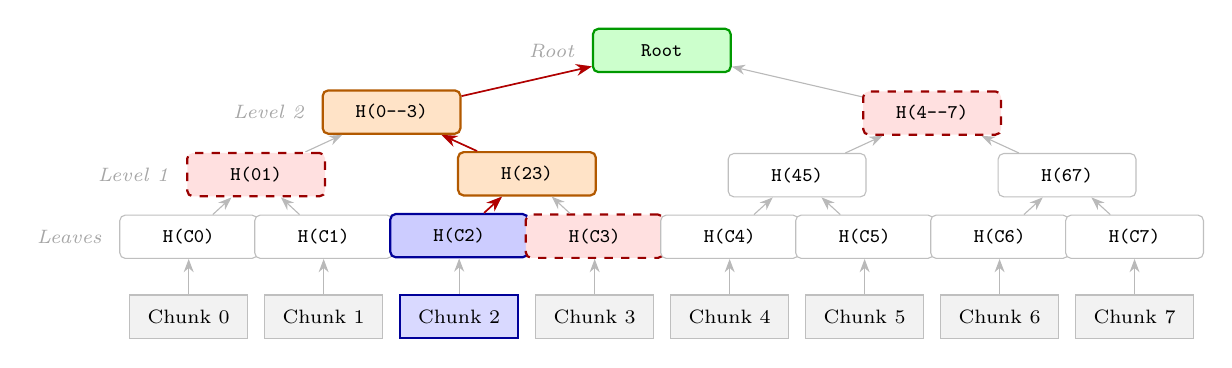
\begin{tikzpicture}[
  node distance=0.55cm and 0.3cm,
  >=Stealth,
  % one reusable base style; all colors inlined per-node below
  N/.style={rectangle, rounded corners=2pt, minimum width=1.75cm,
            minimum height=0.55cm, font=\scriptsize\ttfamily, inner sep=2pt},
  C/.style={rectangle, minimum width=1.5cm, minimum height=0.55cm,
            font=\scriptsize, inner sep=2pt},
  earr/.style={->, gray!55, thin},
  parr/.style={->, red!70!black, semithick},
]

%% ── Chunks ────────────────────────────────────────────────────────
\node[C, draw=gray!50, fill=gray!10]                  (c0) {Chunk 0};
\node[C, draw=gray!50, fill=gray!10, right=0.2cm of c0] (c1) {Chunk 1};
\node[C, draw=blue!60!black, fill=blue!15, thick,
      right=0.2cm of c1]                              (c2) {Chunk 2};
\node[C, draw=gray!50, fill=gray!10, right=0.2cm of c2] (c3) {Chunk 3};
\node[C, draw=gray!50, fill=gray!10, right=0.2cm of c3] (c4) {Chunk 4};
\node[C, draw=gray!50, fill=gray!10, right=0.2cm of c4] (c5) {Chunk 5};
\node[C, draw=gray!50, fill=gray!10, right=0.2cm of c5] (c6) {Chunk 6};
\node[C, draw=gray!50, fill=gray!10, right=0.2cm of c6] (c7) {Chunk 7};

%% ── Leaf hashes ───────────────────────────────────────────────────
\node[N, draw=gray!50,        fill=white,   above=0.45cm of c0] (h0) {H(C0)};
\node[N, draw=gray!50,        fill=white,   above=0.45cm of c1] (h1) {H(C1)};
\node[N, draw=blue!60!black,  fill=blue!20, above=0.45cm of c2, thick] (h2) {H(C2)};
\node[N, draw=red!60!black,   fill=red!12,  above=0.45cm of c3, thick, dashed] (h3) {H(C3)};
\node[N, draw=gray!50,        fill=white,   above=0.45cm of c4] (h4) {H(C4)};
\node[N, draw=gray!50,        fill=white,   above=0.45cm of c5] (h5) {H(C5)};
\node[N, draw=gray!50,        fill=white,   above=0.45cm of c6] (h6) {H(C6)};
\node[N, draw=gray!50,        fill=white,   above=0.45cm of c7] (h7) {H(C7)};

%% ── Level 1 ───────────────────────────────────────────────────────
\node[N, draw=red!60!black,    fill=red!12,    thick, dashed,
      above=0.5cm of $(h0)!0.5!(h1)$]  (n01) {H(01)};
\node[N, draw=orange!70!black, fill=orange!22, thick,
      above=0.5cm of $(h2)!0.5!(h3)$]  (n23) {H(23)};
\node[N, draw=gray!50,         fill=white,
      above=0.5cm of $(h4)!0.5!(h5)$]  (n45) {H(45)};
\node[N, draw=gray!50,         fill=white,
      above=0.5cm of $(h6)!0.5!(h7)$]  (n67) {H(67)};

%% ── Level 2 ───────────────────────────────────────────────────────
\node[N, draw=orange!70!black, fill=orange!22, thick,
      above=0.5cm of $(n01)!0.5!(n23)$] (n03) {H(0--3)};
\node[N, draw=red!60!black,    fill=red!12,    thick, dashed,
      above=0.5cm of $(n45)!0.5!(n67)$] (n47) {H(4--7)};

%% ── Root ──────────────────────────────────────────────────────────
\node[N, draw=green!60!black, fill=green!20, thick,
      above=0.5cm of $(n03)!0.5!(n47)$] (root) {\textbf{Root}};

%% ── All tree edges (gray, drawn before path arrows) ───────────────
\foreach \src/\dst in {c0/h0, c1/h1, c2/h2, c3/h3,
                        c4/h4, c5/h5, c6/h6, c7/h7}
  \draw[earr] (\src)--(\dst);
\draw[earr](h0)--(n01); \draw[earr](h1)--(n01);
\draw[earr](h2)--(n23); \draw[earr](h3)--(n23);
\draw[earr](h4)--(n45); \draw[earr](h5)--(n45);
\draw[earr](h6)--(n67); \draw[earr](h7)--(n67);
\draw[earr](n01)--(n03); \draw[earr](n23)--(n03);
\draw[earr](n45)--(n47); \draw[earr](n67)--(n47);
\draw[earr](n03)--(root); \draw[earr](n47)--(root);

%% ── Proof-path arrows (thick red, drawn last = on top) ────────────
\draw[parr] (h2)--(n23);
\draw[parr] (n23)--(n03);
\draw[parr] (n03)--(root);

%% ── Level labels ──────────────────────────────────────────────────
\node[font=\scriptsize\itshape, text=gray!70, left=0.1cm of h0]   {Leaves};
\node[font=\scriptsize\itshape, text=gray!70, left=0.1cm of n01]  {Level 1};
\node[font=\scriptsize\itshape, text=gray!70, left=0.1cm of n03]  {Level 2};
\node[font=\scriptsize\itshape, text=gray!70, left=0.1cm of root] {Root};

\end{tikzpicture}

\smallskip
{\scriptsize
\begin{tabular}{@{}l@{\hspace{6pt}}l@{\hspace{14pt}}l@{\hspace{6pt}}l@{}}
  \fcolorbox{blue!60!black}{blue!20}{\phantom{xx}} & Verified leaf (H(C2)) &
  \fcolorbox{orange!70!black}{orange!22}{\phantom{xx}} & Recomputed by verifier \\[2pt]
  \fcolorbox{red!60!black}{red!12}{\phantom{xx}}\,\textit{dashed} & Witness (given by prover) &
  \fcolorbox{green!60!black}{green!20}{\phantom{xx}} & Verified root \\
\end{tabular}}

\caption{Merkle tree over an 8-chunk dataset. To verify Chunk~2 the verifier
hashes it to get H(C2)~\textcolor{blue!60!black}{(blue)}, is given the three
\textcolor{red!60!black}{dashed witness hashes} H(C3), H(01), and H(4--7), and
\textcolor{orange!70!black}{recomputes} H(23) and H(0--3) bottom-up along the
bold red arrows ($O(\log N)=3$ steps) until reaching the signed root---without
reading any other chunk data.}
\label{fig:merkle}
\end{figure}


\subsection{Hash Algorithm Selection}

We propose evaluating three hash functions to span the
performance--compliance--standards space:

\begin{itemize}[nosep]
  \item \textbf{SHA-256}: Widely used, FIPS-approved, hardware-accelerated via
    SHA-NI (x86) and SHA extensions (ARM). HMAC-SHA-256 is already identified
    in the S2-D2 proposal for streaming signatures.
  \item \textbf{BLAKE3}~\cite{blake3}: Designed for parallelism---the internal
    tree structure of BLAKE3 maps naturally to a Merkle tree, and it achieves
    $\sim$4$\times$ higher throughput than SHA-256 on modern CPUs without
    hardware acceleration. BLAKE3's built-in tree hashing mode could eliminate
    the need for an external Merkle structure for the per-dataset case.
  \item \textbf{KangarooTwelve}~\cite{k12}: A SHA-3-family parallel hash
    derived from \texttt{Keccak-p}, included as a parallel alternative in
    environments where SHA-256 throughput is the bottleneck. Note that K12 is
    \emph{not} FIPS-approved (only SHA-3-256/384/512 and SHAKE128/256 are FIPS
    202 listed); it is therefore limited to non-FIPS deployments. Its 12-round
    permutation provides a generous security margin while exploiting SIMD and
    multi-core parallelism on long inputs.
\end{itemize}

\noindent The research will benchmark all three on representative scientific
data to determine the performance--compliance tradeoff (SHA-256 for FIPS-required
environments, KangarooTwelve for SHA-3-family parallel deployments where FIPS
is not a constraint, BLAKE3 for maximum throughput where compliance is
unconstrained).

\subsection{Verifiable Subset Extraction}
\label{sec:subset}

A central use case for FAIR scientific data sharing is partial data delivery:
a recipient requests a hyperslab (e.g., a spatial region or temporal window) of
a published dataset, and must be able to verify cryptographically that the
delivered bytes are a true, unmodified subset of the signed parent dataset. A
flat per-dataset hash cannot answer this question without delivering the
entire dataset; per-chunk AEAD authentication can verify that each delivered
chunk is intact \emph{individually}, but cannot prove that the delivered set
constitutes the requested hyperslab and that no requested chunks were silently
omitted, substituted from a different version, or reordered. Note that raw
Merkle inclusion proofs alone also cannot prove coverage: they establish
\emph{membership} (this chunk is in the tree), not \emph{completeness} (all
required chunks were delivered). Coverage is a property of the
\emph{grid hash~$+$~Merkle path} combination described below: the Merkle path
anchors the trusted chunk-grid parameters from the object header, which then
determine exactly which chunks must be present for a given hyperslab request.

This proposal elevates \emph{verifiable subset extraction} to a
first-class research contribution. We define:

\begin{description}[nosep]
  \item[\texttt{extract\_subset(D, H)} $\rightarrow (\mathcal{C}, \pi)$:] given
    a signed dataset~$D$ and a hyperslab~$H$, produce the chunk set
    $\mathcal{C}$ covering~$H$ and a \emph{subset proof}~$\pi$.
  \item[\texttt{verify\_subset($\mathcal{C}, H, \pi$, root)} $\rightarrow \{\bot, \top\}$:]
    accept iff (i)~every chunk in~$\mathcal{C}$ is authenticated by the signed
    root via its Merkle path, (ii)~$\mathcal{C}$ exactly covers the hyperslab
    request~$H$ given the dataset's chunk grid, and (iii)~no chunk in
    $\mathcal{C}$ has been substituted from a different dataset version
    (enforced via the per-chunk version counter, \S\ref{sec:nonce}).
\end{description}

The proof~$\pi$ has three components:
\begin{description}[nosep]
  \item[(a) Merkle witnesses.] The union of Merkle inclusion witnesses for
    every chunk in~$\mathcal{C}$, with shared internal nodes deduplicated.
  \item[(b) Coverage certificate.] The dataset's serialized object header
    (datatype, dataspace dimensionality, chunk grid parameters, and relevant
    attributes) together with its Merkle path to the file-level signed root.
    This allows the recipient to independently verify the trusted chunk-grid
    parameters (via the Merkle path) and then recompute which chunk indices
    \emph{must} have been delivered for hyperslab~$H$.
  \item[(c) Per-chunk version counters.] One 64-bit version counter per chunk
    in~$\mathcal{C}$, bound into each leaf hash and therefore covered by the
    witnesses in (a).
\end{description}

The object header is typically only a few kilobytes, so including it in~$\pi$
is negligible relative to the data payload. The verification workflow is:
(i)~hash the delivered object header; (ii)~verify its Merkle path against
the signed file-level root (using the same proof machinery as chunk
verification); (iii)~extract the trusted chunk-grid parameters; (iv)~use
those parameters to determine which chunk indices cover~$H$; and finally
(v)~verify each chunk's Merkle witness against the signed root. This chain
ensures the recipient cannot be deceived by a poisoned chunk-grid
specification: the grid parameters are covered by the same signature as
the data.

\paragraph{Soundness sketch.}
Define an adversary that wins if it produces $(\mathcal{C}', \pi')$ accepted
by \texttt{verify\_subset} where $\mathcal{C}' \neq \mathcal{C}_H$ (the true
covering set for~$H$). Component~(a) reduces $\mathcal{C}'$ membership soundness
to second-preimage resistance of the underlying hash. Component~(b) reduces
coverage soundness to the integrity of the chunk-grid parameters in the object
header (covered by the file-level root, \S\ref{sec:merkle-storage}).
Component~(c) reduces version-substitution resistance to the binding of $v_k$
into the leaf hash (\S\ref{sec:nonce}). A complete proof---including the
treatment of non-rectangular hyperslabs, partial-chunk requests, and the
interaction with HDF5's filter pipeline---is part of the planned work
(\S\ref{sec:security-analysis}).

\paragraph{Open research questions.}
The proof size~$|\pi|$ grows with both the hyperslab shape and the dataset's
chunk grid. For an $r$-dimensional dataset with $n_i$ chunks per dimension and
a hyperslab touching $m_i$ chunks per dimension, naive witness aggregation
(no deduplication of shared internal nodes) gives
$|\pi| = O\bigl(\prod_i m_i \cdot \log \prod_i n_i\bigr) = O(M \log N)$,
where $M = \prod_i m_i$ is the number of requested chunks and
$N = \prod_i n_i$ is the total chunk count. However, for the
\emph{contiguous dense hyperslabs} that dominate scientific workloads
(rectangular subgrids, time-window selections), shared internal Merkle
nodes can be deduplicated during witness construction.  In the limiting
case of a fully contiguous block, the unique witnesses are concentrated
at the spatial \emph{boundary} of the hyperslab rather than its interior:
proof size scales with the boundary surface area of the requested block,
not its volume, yielding $O\!\left(\mathrm{SurfaceArea}(m_1,\dots,m_r)\cdot\log N\right)$
rather than $O\!\left(\mathrm{Volume}\cdot\log N\right)$,
for axis-aligned hyperslabs under an ideal tree layout (where
$\mathrm{SurfaceArea}(m_1,\dots,m_r)=\sum_i \prod_{j\neq i} m_j$).
\textbf{Important caveat:} the companion dataset stores the Merkle tree in
a 1D linearization of the chunk grid (row-major order by default). A
contiguous hyperslab in a 3D dataset does \emph{not} correspond to a
contiguous range of leaves in this linearization; its leaves are scattered,
so naive deduplication may not recover the surface-area scaling.
Whether an optimized layout can achieve this bound empirically---and what
linearization order best matches common HPC access patterns---is a central
question of RQ6 (\S\ref{sec:research-questions}). For
strided or irregular access patterns (e.g., every 10th time step),
deduplication savings are in general smaller and depend on the companion
dataset's linearization order.

\subsection{Storage of the Merkle Tree}
\label{sec:merkle-storage}

A dataset with $N$ chunks produces a Merkle tree with $\sim 2N$ nodes. Each
node is a 32-byte hash (SHA-256 or BLAKE3). Table~\ref{tab:overhead} shows
storage overhead for representative dataset sizes.

\begin{table}[ht]
\centering
\caption{Merkle tree storage overhead for 32-byte (SHA-256) node hashes.}
\label{tab:overhead}
\begin{tabular}{@{}rrrrr@{}}
\toprule
Dataset Size & Chunk Size & Chunks ($N$) & Tree Size ($\sim 2N \times 32$\,B) & Overhead \\
\midrule
1\,MB   & 64\,KB  & 16       & 1\,KB     & 0.1\%   \\
1\,GB   & 1\,MB   & 1,024    & 64\,KB    & 0.006\% \\
1\,TB   & 1\,MB   & 1,048,576 & 64\,MB   & 0.006\% \\
1\,TB   & 4\,MB   & 262,144  & 16\,MB    & 0.0015\% \\
1\,PB   & 16\,MB  & 67,108,864 & 4\,GB   & 0.0004\% \\
\bottomrule
\end{tabular}
\end{table}

\noindent Note that HDF5 uses fixed-size chunks for each dataset---all chunks
have the same dimensions, so the Merkle tree has uniform leaves by
construction. The overhead calculations above are therefore exact (not
estimates) for any given chunk size and dataset size. Across different datasets
within the same file, chunk sizes may vary, but each dataset's Merkle tree is
independent.

To prevent second-preimage structural attacks (where a crafted chunk payload
matches the 64-byte concatenation of two internal node hashes and is
misinterpreted as an internal node), all hash inputs use \textbf{domain
separation prefixes}: \texttt{0x00} is prepended before hashing leaf inputs,
\texttt{0x01} before hashing internal node pairs, and \texttt{0x02} for
unallocated sparse chunks (preventing a crafted payload from colliding with
the null constant). This makes leaf, internal, and sparse-null hashes
structurally incompatible at the input level, regardless of
the adversary's control over chunk content.

\noindent\textbf{Sparsity side-channel note.}
For unencrypted or publicly readable datasets, the deterministic null
constant $H(\texttt{0x02}\,\|\,\texttt{null})$ is an acceptable and
efficient sentinel. However, for \emph{encrypted} datasets where
confidentiality of structure is required, the positions of null leaves in
the companion Merkle tree are visible to any reader and directly reveal the
physical sparsity pattern of the dataset---potentially leaking sensitive
information (e.g., the shape of sparse genomic or radar data implies content).
If structure-hiding is required, the null hash should instead incorporate a
secret value derived from the dataset encryption key
(e.g., $H(\texttt{0x02}\,\|\,\text{PRF}(\text{DEK},\texttt{"null"}))$),
or the dataset must be allocated as fully dense. This trade-off is noted as
a configuration concern in the security design document.

\noindent An important constraint shapes the storage design: HDF5 attributes
reside in the dataset's object header and are loaded whenever the dataset is
opened, whether the reader needs the attribute or not. For a dataset with one
million 1\,MB chunks, the 64\,MB Merkle tree would bloat the object header
unacceptably. Compact dataset storage has the same problem---it places data
inside the object header and is designed for payloads under $\sim$64\,KB.
Furthermore, storing the tree as an attribute precludes hyperslab access to
individual tree nodes, defeating the $O(\log N)$ partial-verification promise.

We therefore propose a \textbf{hybrid approach} as the recommended storage
design:

\begin{enumerate}[nosep]
  \item A small \textbf{HDF5 attribute} (\texttt{\_merkle\_root}) on the
    dataset containing: the root hash (32\,bytes), the hash algorithm
    identifier (e.g., \texttt{sha256} or \texttt{blake3}), the path to the
    companion dataset, and a \textbf{companion integrity hash}---a hash of
    the serialized companion dataset that anchors the full tree's integrity
    to the signed root. This attribute is lightweight enough to impose
    negligible object header overhead and enables \emph{instant root
    verification}: a reader rehashes the data chunks, recomputes the root, and
    compares---without loading the full tree. The companion integrity hash
    closes a potential attack vector where an adversary modifies internal tree
    nodes in the companion dataset without altering the root, which could
    cause partial verification to accept tampered chunks
    (see~\S\ref{sec:threat}, threat~T1).
  \item A \textbf{chunked companion dataset} (e.g.,
    \texttt{/\_merkle/temperatures}) storing the complete tree as a 1D byte
    array with its own chunked layout (e.g., 4\,KB chunks for fine-grained
    access to 32-byte nodes). This provides:
    \begin{itemize}[nosep]
      \item Hyperslab access to individual proof-path nodes ($O(\log N)$
        positions) without loading the entire tree---critical for partial
        verification performance.
      \item No object header bloat on the parent dataset.
      \item Independent chunk tuning for the tree's I/O pattern.
      \item Natural extensibility: appending chunks to the data dataset appends
        corresponding nodes to the companion dataset, using the same
        incremental I/O pattern.
    \end{itemize}
\end{enumerate}

\noindent For \textbf{small datasets} (under 256 chunks / $\sim$16\,KB of tree),
the full tree may be stored directly in the attribute, avoiding the overhead of
a companion dataset. The implementation will select the appropriate strategy
automatically based on chunk count.

\paragraph{Portability consideration.}
The companion dataset approach has one disadvantage: a reader unaware of the
Merkle convention will see an extra dataset and ignore it, and a na\"{\i}ve
file copy that omits the \texttt{\_merkle} group breaks verification. The root
hash attribute mitigates this---it travels with the dataset and still enables
root-level integrity checking even if the companion is lost. The design
document (\S\ref{sec:impl}, Phase~2) will specify conventions for tools to
preserve companion datasets during copy and subset operations.

\noindent\textbf{Downgrade-to-plaintext threat.}
This \emph{fail-open} default is intentional for backward compatibility but
creates an active attack surface: a compromised storage node or
Man-in-the-Middle can strip the \texttt{\_merkle\_root} attribute and the
\texttt{/\_merkle\_global} companion dataset, causing an unaware reader to
process tampered data without error. To close this gap, the S2-D2 framework's
Data Protection Factory will enforce a \textbf{Strict Mode}: when a file is
known to be governed by a provenance policy (via out-of-band trust metadata,
filesystem extended attributes, or a policy registry), the \emph{absence} of
a valid Merkle root is treated as a fatal security exception rather than a
graceful degradation. Strict Mode is opt-in for interoperability but mandatory
in high-assurance deployment contexts.

\paragraph{Crash consistency.}
The hybrid storage layout introduces a write-ordering requirement: if the
application crashes after writing an encrypted chunk but before updating the
companion Merkle dataset, the tree becomes inconsistent with the data. The
required write-ordering protocol is:
\begin{enumerate}[nosep]
  \item Write the chunk data to disk (via the filter pipeline).
  \item Write the updated Merkle tree nodes to the companion dataset
    (leaf hash, then recomputed path to root).
  \item Update the root attribute (root hash, companion integrity hash,
    and dataset version number).
\end{enumerate}
\noindent Steps 2 and~3 must be flushed before the write is considered
committed. On recovery after a crash, the system detects the inconsistency
(the root attribute will not match the companion dataset state). The recovery
behavior depends on the signing context:

\begin{itemize}[nosep]
  \item \textbf{Unsigned datasets}: The tree may be rebuilt by rehashing the
    on-disk chunk data, since no authenticity guarantee was in force.
  \item \textbf{Signed datasets}: The system must \textbf{fail closed}---report
    the inconsistency and refuse to auto-rebuild. The risk differs by role:
    a \emph{verifier} without the private key cannot re-sign anything and
    simply reports the inconsistency and halts. A \emph{writer} with the private
    key (or with auto-signing enabled) faces the laundering risk: if the runtime
    automatically rehashes on-disk data and signs the result, it would compute
    and sign a new root over potentially tampered chunks, institutionalizing the
    corruption. In both cases the system flags the affected chunks as unverified
    and requires explicit operator intervention (re-signing from a trusted source
    or restoring from a known-good backup).
\end{itemize}

\noindent The C~HDF5 design document (\S\ref{sec:impl}, Phase~2) will specify
this protocol in detail, including interaction with HDF5's existing metadata
journaling and flush semantics, and whether a cryptographic write-ahead log
can provide stronger crash recovery guarantees for signed datasets without the
blind-signing risk.

\subsection{Filter Pipeline Interaction}
\label{sec:filter-order}

The position of hash computation in the filter pipeline has security
implications. We propose the following ordering as the default:

\begin{center}
\texttt{Application data}
$\xrightarrow{\text{shuffle}}$
$\xrightarrow{\text{compress}}$
$\xrightarrow{\text{encrypt}}$
$\xrightarrow{\textbf{hash (Merkle leaf)}}$
\texttt{Storage}
\end{center}

\noindent This is an \emph{Encrypt-then-MAC} (EtM) construction, which is the
standard cryptographic best practice for authenticated encryption and offers
two important properties:

\begin{itemize}[nosep]
  \item \textbf{Third-party integrity verification without decryption.}
    Because the Merkle leaf hashes cover the ciphertext, any party---a storage
    node, middleware, archival system, or researcher without the decryption
    key---can verify that stored chunks have not been modified. This is
    critical for data custody workflows where the verifier is not the data
    owner.
  \item \textbf{Early rejection of tampered ciphertext.}
    A reader encountering modified ciphertext can detect the tampering
    \emph{before} spending CPU cycles on decryption. Under a
    Hash-then-Encrypt ordering, the reader must decrypt the (potentially
    attacker-controlled) ciphertext before discovering via the hash that the
    plaintext is invalid---wasting cycles and expanding the attack surface.
\end{itemize}

\paragraph{Trade-off: plaintext provenance.}
EtM hashes the ciphertext, not the plaintext. This means that rotating the
encryption key (re-encrypting the same data with a new key) changes the
ciphertext and invalidates the Merkle tree, requiring a full tree
recomputation. If plaintext-stable provenance is strictly required (e.g., to
allow key rotation without rebuilding the tree, or to prove that two
differently-encrypted copies contain the same data), a secondary plaintext hash
can be stored alongside the primary ciphertext-based tree. The implementation
will support both orderings, with EtM as the default and
Hash-then-Encrypt available via an explicit configuration flag, along with a
clear warning that the HtE mode sacrifices early tamper rejection and
third-party verifiability.

This ordering will be validated experimentally by measuring verification
correctness and performance for both permutations.

\subsection{Nonce Derivation for Stream Ciphers}
\label{sec:nonce}

Both AES-256-CTR and ChaCha20 are stream ciphers that generate a pseudorandom
keystream XORed with the plaintext. If a chunk is updated in place using the
same symmetric key and the same nonce/IV, the keystream is reused: an attacker
who observes both the old ciphertext $C_\text{old} = P_\text{old} \oplus KS$
and the new ciphertext $C_\text{new} = P_\text{new} \oplus KS$ can compute
$C_\text{old} \oplus C_\text{new} = P_\text{old} \oplus P_\text{new}$,
destroying confidentiality. This is a \textbf{catastrophic vulnerability} if
the nonce is derived statically from the chunk index alone.

To safely support in-place updates, we derive the nonce as:
\begin{equation}
  \text{Nonce}(k, v) = \text{KDF}(\text{DEK}, \; k \,\|\, v)
  \label{eq:nonce}
\end{equation}
where $k$ is the chunk index, $v$ is a monotonically increasing
\textbf{per-chunk version counter}, and DEK is the per-dataset Data Encryption
Key described in~\S\ref{sec:signing}. The version counter is stored in the
companion Merkle dataset alongside the tree nodes (one 64-bit counter per
leaf, adding 8\,bytes per chunk of overhead). Every write to chunk~$k$---whether
an append or an in-place update---increments $v$, guaranteeing a unique nonce
per (key, chunk, version) triple. The version counter also serves double duty
for rollback detection (threat~T4 in~\S\ref{sec:threat}): the dataset-level
version in the signed root is the maximum of all per-chunk versions, providing
a monotonic timeline. The locally stored high-resolution timestamp~$\tau$
in the signed payload~$R$ similarly defends against T4 by making rollback
detectable to any verifier with a prior observation. However, it is important
to note that \textbf{local timestamps provide no protection against key
compromise}: an attacker who obtains the Ed25519 private key can generate a
freshly signed payload with a backdated~$\tau$, fabricating an apparently old
provenance record. True non-repudiation and key-compromise resilience require
an \emph{external} cryptographic timestamp from a trusted Timestamp Authority
(TSA, RFC~3161~\cite{rfc3161}), which is why the Sigstore~$+$~TSA token
stretch goal (\S\ref{sec:signing}) is architecturally significant and not
merely a deployment convenience.

An alternative is to generate a fully random nonce per write and store it
alongside the ciphertext. This avoids the need for a persistent counter but
increases per-chunk storage overhead and introduces a dependency on the quality
of the random number generator. The implementation will support both schemes,
with the version-counter approach as the default.

\subsection{Signing Authority and Key Management}
\label{sec:signing}

A Merkle tree without a signed root is vulnerable to wholesale replacement (an
attacker replaces both data and tree; see threat~T1 in~\S\ref{sec:threat}). The
core signing mechanism is:

\begin{itemize}[nosep]
  \item The file creator signs the root hash (and the companion integrity hash)
    with an \textbf{Ed25519 private key}. Ed25519 is chosen for its fast
    verification, small signature size (64~bytes), and resistance to
    timing side-channels. The signed payload includes the dataset version
    number and a high-resolution timestamp to defend against rollback attacks
    (threat~T4).
  \item The corresponding public key is distributed via one of two mechanisms:
    (a)~embedded in a file attribute (\texttt{\_provenance\_pubkey}) for
    self-contained verification, or (b)~distributed via the Task~2 KeyStore
    (\texttt{HDF5\_PLUGIN\_KEYSTORE\_DIR} / \texttt{HDF5\_PLUGIN\_KEYSTORE}),
    reusing the trusted-key infrastructure from PR~\#6198.
\end{itemize}

\paragraph{Post-quantum hybrid signing (T5: harvest-now, forge-later).}
\label{sec:pq-hybrid}
Scientific data is routinely retained for decades---NOAA climate baselines,
EQSIM simulation outputs, genomic reference assemblies, and astronomical
survey data are all held on archival timescales of 30--100~years. Within that
horizon, a cryptographically relevant quantum computer (CRQC) is widely
expected to render Ed25519 (and all elliptic-curve and RSA signatures)
forgeable via Shor's algorithm. An adversary who archives today's signatures
and waits---the \emph{harvest-now, forge-later} threat (T5)---can later
fabricate signed roots over tampered datasets attributed to the original
signer. This proposal therefore promotes \textbf{post-quantum hybrid signing}
to a first-class research deliverable. The signed root attribute carries a
hybrid signature consisting of:

\begin{equation}
  \sigma_\text{root} = \bigl(\sigma_\text{Ed25519}(R), \;
                            \sigma_\text{ML-DSA-65}(R)\bigr),
  \quad R = \text{root} \,\|\, \text{companion\_hash} \,\|\, v_\text{dataset} \,\|\, \tau \,\|\, \text{AlgID}
\end{equation}

\noindent where $R$ is the canonical signed payload (root, companion integrity
hash, dataset-level version counter, timestamp, and a compact algorithm
identifier). Including \textbf{AlgID}---a fixed-width encoding of the hash
function (e.g., \texttt{BLAKE3}) and AEAD cipher (e.g.,
\texttt{ChaCha20-Poly1305}) in use---prevents \emph{Algorithm Substitution
Attacks}: an attacker who rewrites the \texttt{\_merkle\_root} attribute to
specify a weaker hash or cipher cannot produce a valid signature over the
modified payload, because the algorithm identifiers are covered by both
$\sigma_\text{Ed25519}$ and $\sigma_\text{ML-DSA-65}$. ML-DSA-65 (NIST FIPS
204~\cite{fips204}) is NIST PQC Category~3, providing approximately AES-192
strength against both classical and quantum attacks; SLH-DSA-128s (NIST FIPS 205~\cite{fips205}) is also
implemented as an alternative for deployments preferring hash-based
signatures whose security rests only on the underlying hash function. A
verifier accepts the signature iff \emph{both} components verify
(strict-AND policy). This means that even today---before a CRQC exists---a
verifier will reject if either signature is invalid; a file signed with
Ed25519 alone will not be accepted. This is intentional: it prevents a
downgrade attack where an adversary strips the PQ component. Until a CRQC
exists, Ed25519 dominates verification time (ML-DSA-65 verification is
somewhat slower); once a CRQC exists, the ML-DSA-65 component preserves
authenticity while the Ed25519 component is considered compromised.

\paragraph{One signature, all datasets.}
The hybrid signature is applied \textbf{once} to the global
\emph{file-level} root that aggregates all per-dataset roots
(\S\ref{sec:merkle-storage}). Individual datasets contribute a
32-byte hash to the global tree; they do not each carry a
3.3~KB~ML-DSA-65 signature. For a file with $10^5$ datasets,
the total signing overhead is one 3.3~KB signature (plus a $\sim$2~KB
public key) stored in a single file-level attribute, not $10^5 \times
3.3$~KB~$= 330$~MB spread across per-dataset object headers. Signing
and verifying an individual dataset at rest still requires only
$O(\log D)$ hash reads from the companion tree (where $D$ is the
number of datasets in the file), never a per-dataset PQ signature.
The file-level tree nodes are stored in a dedicated companion dataset
at the HDF5 file root (e.g., \texttt{/\_merkle\_global}), using the
same chunked-companion layout as per-dataset trees (\S\ref{sec:merkle-storage}),
so the global tree itself imposes no object-header overhead.

\paragraph{Why this still needs to be measured at HDF5 scale.}
ML-DSA-65 signatures are $\sim$3.3~KB and public keys are $\sim$2~KB, versus
64~B and 32~B for Ed25519. SLH-DSA signatures are larger still ($\sim$8~KB
to $\sim$30~KB depending on parameters). Even with a single file-level
signature, the \emph{object-header encoding} of the file-level root attribute
(which contains the root hash, companion integrity hash, version counter,
timestamp, and the hybrid signature blob) must remain within HDF5's
attribute-storage limits. HDF5 object headers begin failing silently past
$\sim$64~KB and cannot accommodate 330~MB. Verifying that the
file-level root attribute stays within these limits for all supported
parameter combinations, and measuring batch verification throughput at
$10^4$--$10^7$ chunks (covering 10\,GB--10\,TB datasets at 1\,MB chunk size), is the substance of RQ7
(\S\ref{sec:research-questions}) and is intended to be a primary empirical
contribution of the resulting paper, supplying the first published
PQ-signature performance numbers for scientific data archives.

\paragraph{Symmetric key management.}
The asymmetric Ed25519 key provides signing (authenticity), but the encryption
layer (AES-256-CTR, ChaCha20-Poly1305) requires symmetric Data Encryption Keys
(DEKs). The full design of key management is a broader S2-D2 concern (spanning
Tasks~2 and~3); for the ClawHDF5 prototype, we adopt the following baseline
scheme: a single DEK per dataset is generated at dataset creation, wrapped
(encrypted) with a Key Encryption Key (KEK) derived from user credentials via
HKDF-SHA-256, and stored as an HDF5 attribute
(\texttt{\_provenance\_wrapped\_dek}) on the dataset. The KEK is never stored
in the file. This supports the common case where one user or group encrypts a
dataset; multi-party access (multiple KEKs wrapping the same DEK) and external
KMS integration are deferred to the C~HDF5 design document.

\paragraph{AEAD integration.}
When ChaCha20-Poly1305 is used, the cipher natively produces a 16-byte
Poly1305 authentication tag per chunk. To avoid discarding this tag (which
would waste a security property the cipher already provides), the Merkle leaf
hash for a ChaCha20-Poly1305-encrypted chunk is computed over the
concatenation of the ciphertext and the Poly1305 tag:
\begin{equation}
  H_\text{leaf}(k) = H(\texttt{0x00} \,\|\, k \,\|\,
                        \text{Ciphertext}_k \,\|\, \text{Tag}_k \,\|\, v_k),
\end{equation}
where $v_k$ is the per-chunk version counter (\S\ref{sec:nonce}) and
$\texttt{0x00}$ is the leaf domain-separation prefix (\S\ref{sec:merkle-storage}).
Explicitly binding the chunk index~$k$ into the leaf hash prevents
\emph{position-swapping attacks}: an adversary cannot substitute the
ciphertext, tag, and version counter of chunk~$k'$ in place of chunk~$k$,
because the index is baked into the hash; the forged leaf will not match
the honest leaf at position~$k$ in the tree, and Merkle path verification
will reject it. This is especially important under Sparse Merkle Trees,
where dynamically collapsed subtrees could otherwise introduce structural
ambiguity in proof generation. Critically, including $v_k$ in the leaf hash
\textbf{cryptographically binds the version counter to the tree}: if an
attacker selectively rolls back a chunk and its corresponding version counter
in the companion dataset, the leaf hash changes, breaking the path to the
signed root. For AES-256-CTR (which is not an AEAD cipher), the HMAC-SHA-256
authentication tag serves an analogous role:
$H(\texttt{0x00} \,\|\, k \,\|\, \text{Ciphertext}_k \,\|\, \text{HMAC}_k \,\|\, v_k)$.
For \emph{plaintext} (unencrypted) chunks, the leaf hash binds the raw chunk
data and version counter directly:
$H(\texttt{0x00} \,\|\, k \,\|\, \text{Chunk}_k \,\|\, v_k)$;
the index~$k$ is bound in all cases to prevent position-swapping attacks.

\paragraph{Stretch goal: Sigstore transparency log.}
As an extension, the signed root may be published to a
\textbf{Sigstore transparency log}~\cite{newman2022sigstore,
laurie2014certificate}, establishing a public, append-only audit trail of who
signed what and when. This extends Task~3 provenance with a public,
tamper-evident audit trail and is independent of Task~2's plugin-signing
KeyStore (which does not use Sigstore). A practical consideration: Sigstore uses short-lived certificates
issued via OIDC/Fulcio, which means the certificate will have expired by the
time a researcher verifies the dataset months or years later. The
implementation must therefore store the \textbf{Rekor inclusion proof}
(transparency log bundle) as an HDF5 attribute alongside the signature, enabling
offline verification against the log's Merkle root without requiring the
original certificate to still be valid. For datasets archived for decades---a
common requirement in scientific data management---institutional domain changes
may render OIDC identity verification ambiguous. To support
\textbf{Long-Term Validation} (LTV), the implementation will also store a
trusted \textbf{Timestamp Authority} (TSA) token~\cite{rfc3161} alongside the
Rekor bundle. The TSA token mathematically proves the signature occurred before
the certificate expired, ensuring cryptographic validity for 50+ years
independent of the signer's institutional identity. Sigstore integration
involves external service dependencies and is therefore scoped as a stretch goal
for Phase~2 (\S\ref{sec:impl}).

\subsection{Security Analysis Methodology}
\label{sec:security-analysis}

A central weakness of prior provenance-style systems papers is that the
security claim is asserted by intuition rather than argued formally,
inviting reviewer rejection at security venues and leaving operational
deployments without a defensible model. We therefore commit to producing
either a symbolic protocol model or a game-based argument as part of this
research:

\begin{description}[nosep]
  \item[Game-based argument (baseline, in scope).]
    A written argument in the paper showing that the construction
    \mbox{(EtM~filter pipeline)~$+$~(version-counter nonce)~$+$~(hybrid
    signed root over companion-integrity hash)} achieves
    \emph{verified-subset soundness} (an EUF-CMA-style goal over the
    authenticated data structure: no adversary can produce an accepted
    $(\mathcal{C}', \pi')$ that differs from the honest covering set) against
    the adversary defined in \S\ref{sec:threat}, by reduction to
    (a)~the second-preimage resistance of the underlying hash function,
    (b)~the EUF-CMA security of the hybrid signature scheme, and
    (c)~the per-chunk INT-CTXT security already provided by the AEAD cipher
    (for encrypted datasets) or by the Merkle leaf hash alone (for plaintext
    datasets). Note that the Merkle layer does not re-derive INT-CTXT at the
    chunk level---AEAD ciphers such as ChaCha20-Poly1305 already provide this
    via their authentication tag; instead, the Merkle layer adds
    \emph{cross-chunk and cross-version binding} that no per-chunk AEAD can
    provide. We follow the Bellare--Namprempre framework for analyzing generic
    composition~\cite{bellare2000encrypt}.
  \item[Symbolic model (stretch, preferred for security venues).]
    A Tamarin Prover~\cite{meier2013tamarin} model of the file-creation,
    update, and verification protocols, including the version-counter
    binding into leaf hashes and the hybrid-signature root, with
    machine-checked verification of the principal security lemmas
    (authenticity, freshness, subset soundness). Because Tamarin is
    designed for finite protocol state machines and does not natively
    handle unbounded recursive data structures, the model will prove
    lemmas over a \textbf{depth-bounded instantiation} of the tree
    (e.g., depth $d \leq 30$, covering trees of up to $10^9$ chunks).
    Security at arbitrary depth is argued by structural induction over the
    depth-bounded proof, a standard technique in symbolic tree analysis.
    The Tamarin model and all proof scripts would be released alongside
    the implementation.
\end{description}

\noindent The game-based argument is treated as a Phase~2 deliverable; the
Tamarin model is a stretch deliverable whose completion would target a
security venue (USENIX Security, ACSAC) for the resulting paper.

\subsection{Research Questions}
\label{sec:research-questions}

\begin{enumerate}[label=\textbf{RQ\arabic*}]
  \item What is the storage overhead of Merkle trees as a function of chunk
    size and dataset size, and at what chunk count does the hybrid
    companion-dataset approach outperform attribute-only storage in terms of
    object header impact and partial verification access time?
  \item What is the partial verification latency for realistic scientific
    access patterns (sequential scan, strided hyperslab, random chunk access)
    compared to full-dataset rehashing?
  \item How does incremental tree extension perform for append-heavy workloads
    (time-series, streaming sensor data) compared to re-signing the entire
    dataset?
  \item What is the throughput advantage of BLAKE3 and KangarooTwelve over
    SHA-256 for Merkle tree construction at HDF5-typical chunk sizes, and does
    BLAKE3's internal tree hashing mode offer additional speedup for
    whole-dataset root computation? (Note: BLAKE3's internal tree uses fixed
    1\,KB leaf chunks and does not expose intermediate nodes via its public
    API, so it cannot replace the external Merkle structure for partial
    verification. This question is therefore scoped to throughput comparison,
    not structural subsumption.)
  \item Can the Merkle tree detect and localize tampering injected into
    specific chunks of real-world scientific datasets (NOAA climate, EQSIM
    simulation~\cite{mccallen2021eqsim})?
  \item \textbf{(Subset extraction.)}~What is the achievable proof
    size~$|\pi|$ for verifiable hyperslab subset extraction
    (\S\ref{sec:subset}) as a function of hyperslab shape (rectangular,
    strided, sparse), dataset chunk grid, and companion-dataset layout, and
    what is the proof-construction and proof-verification latency relative
    to the bandwidth saved over a na\"{\i}ve full-dataset re-download?
  \item \textbf{(Post-quantum signing.)}~What are the storage, sign, and
    verify costs of hybrid Ed25519~$+$~ML-DSA-65 (and Ed25519~$+$~SLH-DSA-128s)
    signed roots at $10^4$--$10^5$ datasets per file and $10^4$--$10^7$
    chunks per dataset (10\,GB--10\,TB at 1\,MB chunk size), including object-header impact and end-to-end
    verification time on x86-64 (with and without AVX-512) and ARM?
  \item \textbf{(Adversarial soundness.)}~Can a white-box adversary with
    full design knowledge and read/write access to the storage medium evade
    detection by the verification protocol within the stated threat model
    (T1--T8)? For each attack class (T1a, T1b, T2--T5, subset-extraction
    attacks), we report: whether the verifier rejects, the tamper-localization
    granularity (which chunks are flagged), and the detection latency. Any
    successful attacks are root-cause-analyzed and the design is updated. This
    is evaluated via the white-box red-team study described
    in~\S\ref{sec:adversarial}.
\end{enumerate}


%% ============================================================================
\section{Experimental Plan}
\label{sec:experiments}

\subsection{Datasets}

We will use publicly available scientific datasets identified in the S2-D2
proposal:

\begin{itemize}[nosep]
  \item \textbf{NOAA Climate Data Online}: Multi-variable gridded climate data,
    representative of regular-access time-series workloads.
  \item \textbf{EQSIM earthquake simulation}~\cite{mccallen2021eqsim}:
    Large-scale simulation output from Lawrence Berkeley National Laboratory,
    representative of HPC checkpoint/restart patterns.
  \item \textbf{Synthetic datasets}: Parameterized by chunk size (64\,KB to
    16\,MB), chunk count ($10^2$ to $10^7$), dimensionality (1D to 3D), and
    compression ratio, for controlled benchmarking.
\end{itemize}

\subsection{Hardware Platforms}

\begin{itemize}[nosep]
  \item \textbf{Workstation}: Modern x86-64 with AVX-512 and SHA-NI for
    hardware-accelerated hashing.
  \item \textbf{ARM platform}: Apple Silicon or AWS Graviton, exercising NEON
    SIMD and ARM SHA extensions.
\end{itemize}

\subsection{Evaluation Baselines}

Beyond comparing Merkle-tree partial verification ($O(\log N)$) against
full-dataset rehashing ($O(N)$)---which is expected to favor the Merkle tree by
construction---we include three additional baselines targeted at the questions
reviewers most often raise:

\begin{description}[nosep]
  \item[Filesystem-level checksumming
    (ZFS~\cite{bonwick2003zfs}, Btrfs).] Addresses
    \emph{``Why do this in HDF5 when my filesystem already prevents silent
    data corruption?''} The answer is that filesystem checksums are stripped
    the moment a file is transferred over a network, uploaded to cloud
    storage, or moved to a different filesystem. Application-level (HDF5)
    Merkle trees \emph{travel with the data} and can be verified by any
    recipient regardless of the underlying storage.
  \item[Cloud object-store checksums (S3 ETag, GCS CRC32C).] Addresses
    \emph{``S3 already gives me per-object integrity.''} Object stores
    expose a flat per-object hash and lack hierarchical structure for
    partial verification, sub-object tamper localization, or
    non-repudiable signing. The cloud baseline (\S\ref{sec:cloud-eval})
    quantifies this gap by comparing proof-of-chunk retrieval over S3
    range-GETs against full-object re-download.
  \item[Per-chunk AEAD only (no Merkle tree).] Addresses
    \emph{``Why not just AEAD every chunk and be done?''} This baseline
    verifies that AEAD alone cannot answer ``has \emph{any} chunk been
    modified?'' without decrypting all chunks, and cannot localize
    tampering without an external authenticated structure.
\end{description}

\subsection{Cloud Object-Store Evaluation}
\label{sec:cloud-eval}

A growing fraction of scientific HDF5 deployments runs over cloud object
stores: HSDS~\cite{hsds}, h5coro~\cite{h5coro}, and the ros3 VFD all access
HDF5 over S3-compatible APIs. The companion-dataset design maps naturally to
this environment: $O(\log N)$ proof-path nodes can be retrieved via
HTTP range-GETs against the companion's chunked layout, without downloading
the data chunks themselves. We evaluate this end-to-end for two cloud
scenarios---intra-region (LAN-class latency) and cross-region (WAN, $\sim$80~ms
RTT)---measuring (a)~bytes transferred for verifying a hyperslab via subset
proof versus full re-download, (b)~wall-clock latency of the proof-then-verify
path, and (c)~the impact of HTTP/2 multiplexing on proof-path retrieval
latency. This is the first reported measurement of authenticated partial
verification for HDF5 over cloud storage, and directly grounds the
``portability'' benefit of application-level Merkle trees in concrete numbers.

\subsection{Adversarial Red-Team Study}
\label{sec:adversarial}

A common failure mode of integrity-system papers is that the ``tamper
detection'' experiment injects modifications using the system's own
write path and then reports near-100\% true-positive / 0\% false-positive
rates. This trivially confirms that the verifier rejects what the writer
breaks; it does not test whether a directed adversary can evade detection.
We instead conduct a \emph{white-box red-team study} in which the adversary
has full design knowledge, full read/write access to the storage medium, and
attempts to mount each threat in \S\ref{sec:threat}:

\begin{description}[nosep]
  \item[T1a (storage-level tampering, data).] Targeted single- and
    multi-chunk modification, including modifications of compressed
    payloads designed to remain valid after the filter pipeline.
  \item[T1b (storage-level tampering, internal tree nodes).] Modification of
    internal nodes in the companion dataset without altering the root,
    targeting the companion-integrity-hash defense
    (\S\ref{sec:merkle-storage}).
  \item[T2 (silent data corruption).] Single-bit and burst-error injection
    via deliberate fault injection on a known-good chunk.
  \item[T3 (provenance forgery).] Substitution of the
    \texttt{\_provenance\_pubkey} attribute alone, and key-confusion attacks
    on the hybrid signature.
  \item[T4 (rollback).] Substitution of an entire valid prior version of the
    file (data, companion, root attribute), and selective per-chunk rollback
    where the chunk and its version counter are both restored to a prior
    valid state. The latter targets the version-counter binding into the
    leaf hash (\S\ref{sec:nonce}).
  \item[T5 (post-quantum).] Simulated forgery of the Ed25519 component of
    the hybrid signature (assuming oracle access to a CRQC), to confirm that
    the ML-DSA-65 component blocks acceptance.
  \item[Subset-extraction attacks.] (a)~Omission of a chunk from the delivered
    set; (b)~substitution of a chunk from a different version; (c)~delivery
    of a covering set that does not match the requested hyperslab.
\end{description}

For each attack class we report whether the verifier rejects, the
proof-of-failure granularity (which chunk(s) were flagged), and the wall-clock
detection latency. Attacks that succeed are root-cause-analyzed and the
design is iterated; this is treated as a research result, not a defect.

\subsection{Metrics}

\begin{itemize}[nosep]
  \item \textbf{Throughput}: MB/s for hash computation
    (SHA-256, BLAKE3, KangarooTwelve) and encryption (ChaCha20-Poly1305)
    at varying chunk sizes.
  \item \textbf{Partial verification latency}: Wall-clock time to verify a
    single chunk via Merkle proof vs.\ full-dataset rehash.
  \item \textbf{Subset-proof size and latency}: $|\pi|$ and end-to-end
    \texttt{extract}/\texttt{verify} time as a function of hyperslab shape.
  \item \textbf{WAN bandwidth savings}: Bytes transferred for proof-of-subset
    over S3 range-GETs vs.\ full re-download.
  \item \textbf{Hybrid-signature cost}: Sign and verify time, signature size,
    public-key size, and object-header impact for Ed25519 alone vs.\
    Ed25519~$+$~ML-DSA-65 vs.\ Ed25519~$+$~SLH-DSA-128s.
  \item \textbf{Incremental update cost}: Time to append $k$ chunks or
    overwrite $k$ existing chunks and update the Merkle tree vs.\ re-signing
    the entire dataset.
  \item \textbf{Storage overhead}: Bytes consumed by Merkle tree, companion
    dataset, version counters, and provenance metadata as a fraction of
    dataset size.
  \item \textbf{Adversarial-evasion rate}: Number of red-team attack classes
    detected vs.\ undetected (\S\ref{sec:adversarial}); for undetected
    attacks, the time-to-fix in the design.
\end{itemize}

\subsection{Statistical Protocol}

Each benchmark configuration will be measured over a minimum of 30 trials
preceded by 5 warmup runs (discarded). We report median and 95th-percentile
latency, with 95\% confidence intervals computed via bootstrapping. To control
for variance from background system activity, benchmarks will be run with CPU
frequency scaling disabled (\texttt{performance} governor), on an isolated set
of cores (via \texttt{taskset}), and with filesystem caches dropped between
trials for I/O-sensitive measurements.


%% ============================================================================
\section{Implementation Plan}
\label{sec:impl}

The implementation plan is structured around the three primary research
contributions identified in the abstract: verifiable subset extraction,
post-quantum hybrid signing, and a security analysis backed by an adversarial
red-team study. Throughout this section, ``Move~$N$'' labels a publication-unit
contribution targeted at the resulting paper (Move~1 = verifiable subset
extraction, Move~2 = PQ hybrid signing, Move~3 = adversarial red-team study,
Move~4 = security analysis, Move~5 = append-only Merkle log, Move~6 = cloud
evaluation). Items not on the critical path to the primary contributions---in
particular AES-256-CTR~$+$~HMAC-SHA-256 filters and live Sigstore service
integration---are deferred to Phase~3 / future work to preserve focus.

\subsection{Phase 1: Core Architecture and Verifiable Subset (Months 1--4)}

\begin{enumerate}[nosep]
  \item \textbf{Platform evaluation (go/no-go, end of Month~1):} Verify that
    ClawHDF5 can open, chunk-iterate, and write back a 10\,GB multi-dataset
    test file. If this gate fails, activate the standalone-library fallback
    (see~\S\ref{sec:risks}).
  \item Add \texttt{MerkleTree} struct to \texttt{clawhdf5-format}, building
    the tree from chunk hashes during write. Evaluate
    \textbf{SHA-256, BLAKE3, and KangarooTwelve} on HDF5-typical chunk sizes
    (RQ4).
  \item Implement the hybrid storage layout: root-hash attribute
    (\texttt{\_merkle\_root}) on the dataset plus chunked companion dataset
    (\texttt{/\_merkle/<name>}) for the full tree, including the
    \emph{companion-integrity hash} bound into the root attribute.
    Include automatic fallback to attribute-only storage for small datasets
    ($\leq 256$ chunks).
  \item Implement the verification API: \texttt{verify\_root}
    (instant root check from attribute alone), \texttt{verify\_chunk}
    (partial verification via proof path, $O(\log N)$ companion reads),
    \texttt{verify\_dataset} (full tree verification), and
    \texttt{extend\_merkle} / \texttt{update\_merkle} for incremental append
    and in-place overwrite along the affected $O(\log N)$ path.
  \item \textbf{Verifiable subset extraction (Move~1):}
    implement \texttt{extract\_subset(dataset, hyperslab)} returning the
    chunk set plus the subset proof~$\pi$ defined in~\S\ref{sec:subset},
    and \texttt{verify\_subset(...)} for the recipient side. Include
    witness deduplication for shared internal nodes and the coverage
    certificate over the dataset's chunk-grid parameters. Empirically
    characterize $|\pi|$ for rectangular, strided, and sparse hyperslab
    shapes (RQ6).
  \item Benchmark against ClawHDF5's existing flat SHA-256 per-dataset
    verification on synthetic and NOAA datasets, measuring companion dataset
    I/O overhead vs.\ attribute-only at varying chunk counts (RQ1, RQ2, RQ3).
\end{enumerate}

\subsection{Phase 2: Security Contributions and Evaluation (Months 4--7)}

\begin{enumerate}[nosep]
  \item \textbf{Hybrid signing (Move~2):} implement
    Ed25519~$+$~ML-DSA-65 signed roots over the canonical payload
    $R = \text{root} \,\|\, \text{companion\_hash} \,\|\, v_\text{dataset}
    \,\|\, \tau \,\|\, \text{AlgID}$ (\S\ref{sec:pq-hybrid}), with Ed25519~$+$~SLH-DSA-128s
    available as an alternative. Measure end-to-end sign/verify cost,
    signature and public-key size, and object-header impact at
    $10^4$--$10^5$ datasets per file and $10^4$--$10^7$ chunks per dataset
    (10\,GB--10\,TB at 1\,MB chunk size; RQ7) on x86-64 (with and without AVX-512) and ARM.
  \item Implement ChaCha20-Poly1305 as the primary AEAD encryption filter,
    including the version-counter-based nonce derivation scheme
    (\S\ref{sec:nonce}) and the AEAD-tag~$+$~version-counter binding into
    the Merkle leaf hash (\S\ref{sec:signing}). The DEK / KEK / HKDF baseline
    key management is implemented to the level required to run encrypted
    end-to-end experiments; the broader key-management design is deferred to
    the C~HDF5 design document.
  \item \textbf{Security analysis (Move~4):} produce the
    Bellare--Namprempre-style game-based argument
    (\S\ref{sec:security-analysis}) for the EtM~$+$~version-counter~$+$
    hybrid-signed-root construction. The Tamarin model is undertaken as a
    stretch deliverable if the schedule permits.
  \item \textbf{Adversarial red-team study (Move~3):} execute the white-box
    attack suite of \S\ref{sec:adversarial} on NOAA and EQSIM datasets,
    covering T1--T8 plus the subset-extraction attack classes. Report the
    detected/undetected matrix and root-cause-analyze any successful attacks.
  \item \textbf{Cloud object-store evaluation (Move~6):} implement the
    companion-dataset proof retrieval over S3 range-GETs (via the existing
    cloud read paths in ClawHDF5) and run the intra-region and
    cross-region WAN measurements of \S\ref{sec:cloud-eval}. The HSDS and
    h5coro APIs serve as deployment references but are not modified as part
    of this work.
  \item Produce a \textbf{design document for C HDF5 integration} specifying:
    Merkle tree hybrid storage format (root-hash attribute plus companion
    dataset, with attribute-only fallback for small datasets), proposed
    HDF5 API additions (\texttt{H5Dverify\_chunk},
    \texttt{H5Dextract\_subset}, \texttt{H5Fget\_integrity\_root}),
    companion dataset preservation semantics for copy/subset operations,
    crash consistency write-ordering protocol (chunk $\to$ companion
    $\to$ root attribute), filter pipeline ordering requirements, and the
    on-disk layout of the hybrid signed-root attribute.
  \item Write an RFC-style document for the HDF5 community.
\end{enumerate}

\subsection{Phase 3 / Stretch}

\begin{enumerate}[nosep, resume]
  \item \textbf{Append-only log Merkle mode (Move~5)}: a
    Certificate-Transparency-style variant supporting consistency proofs
    between dataset versions (\emph{``version $n$ is a true prefix of version
    $m$''}), targeting time-series and streaming science workloads.
  \item \textbf{Tamarin symbolic model} of the verification protocol, with
    machine-checked authenticity, freshness, and subset-soundness lemmas;
    intended to elevate the security analysis from game-based argument to
    machine-checked proof for a security-venue paper submission.
  \item \textbf{Sigstore transparency-log publication} for hybrid signed
    roots, including Rekor inclusion proof storage and RFC~3161 TSA token
    storage for Long-Term Validation.
  \item \textbf{AES-256-CTR~$+$~HMAC-SHA-256 filters} for FIPS-required
    deployments where ChaCha20-Poly1305 is not acceptable.
  \item \textbf{Provenance-graph integration}: bind the Merkle root as a
    W3C PROV~\cite{w3cprov} \texttt{prov:Entity} identifier so that
    derivation chains across datasets reference content-stable, signed
    roots.
\end{enumerate}


%% ============================================================================
\section{Deliverables and S2-D2 Contributions}
\label{sec:deliverables}

\begin{table}[ht]
\centering
\caption{Mapping of deliverables to S2-D2 tasks. The three primary research
contributions targeted at the resulting publication are starred.}
\label{tab:deliverables}
\begin{tabular}{@{}p{7.0cm}ccc@{}}
\toprule
Deliverable & S2-D2 Task & Phase & Scope \\
\midrule
Merkle-tree provenance implementation in ClawHDF5 (hybrid storage,
  companion-integrity-hash)
  & Task 3 & 1 & Core \\
Hash benchmark: SHA-256, BLAKE3, KangarooTwelve at HPC chunk sizes
  & Task 3 & 1 & Core \\
$\star$~Verifiable subset extraction protocol and implementation (Move~1)
  & Task 3 & 1 & Core \\
$\star$~Hybrid Ed25519~$+$~ML-DSA-65 signed roots with PQ measurements
  at HDF5 scale (Move~2)
  & Task 2, 3 & 2 & Core \\
ChaCha20-Poly1305 AEAD filter with version-counter nonce derivation and
  AEAD-tag binding into the Merkle leaf
  & Task 3 & 2 & Core \\
Game-based security argument for EtM~$+$~version-counter~$+$~hybrid-signed-root
  (Move~4)
  & Task 3 & 2 & Core \\
$\star$~Adversarial red-team study on NOAA and EQSIM datasets (T1--T8
  $+$~subset-extraction attacks) (Move~3)
  & Task 3 & 2 & Core \\
Cloud object-store evaluation (S3 range-GET proof retrieval, WAN
  measurements) (Move~6)
  & Task 3 & 2 & Core \\
C HDF5 integration design document and RFC
  & Task 3 & 2 & Core \\
Append-only log Merkle mode with consistency proofs (Move~5)
  & Task 3 & 3 & Stretch \\
Tamarin symbolic model of verification protocol
  & Task 3 & 3 & Stretch \\
Sigstore transparency-log publication with Rekor + TSA storage
  & Task 3 & 3 & Stretch \\
AES-256-CTR + HMAC-SHA-256 filters (FIPS-required deployments)
  & Task 3 & 3 & Stretch \\
PROV~\cite{w3cprov} provenance-graph integration
  & Task 3 & 3 & Stretch \\
\bottomrule
\end{tabular}
\end{table}

\subsection{Contribution to S2-D2 Goals}

\begin{itemize}[nosep]
  \item \textbf{SHINES alignment}: The Merkle-tree prototype implements
    concrete technical mechanisms within the safety/security/privacy taxonomy
    and threat categorization (FMT, LIB, EXT, TCD) established by the HDF5
    SHINES project~\cite{shines}, grounding the vocabulary in working code.
    The post-quantum threat T5 (\S\ref{sec:threat}) extends the SHINES
    taxonomy with a long-archival risk category not yet covered by the
    current vocabulary.
  \item \textbf{Task 2 connection}: Task~2 has implemented RSA plugin
    signature verification in the C HDF5 library (PR~\#6198), introducing a
    \texttt{KeyStore} for trusted public keys, an append-style signature footer
    on plugin binaries, a revocation blocklist, and the \texttt{h5sign}
    command-line signing tool.  The present proposal shares this trust
    infrastructure: dataset-root signing keys can be managed through the same
    KeyStore mechanism, and the post-quantum hybrid pattern introduced here
    (Ed25519~$+$~ML-DSA-65) provides a forward-compatible upgrade path for
    plugin signing on long-archival timescales, without requiring Sigstore
    or any external transparency service.
  \item \textbf{Task 3 contribution}: The Merkle tree provides a concrete,
    benchmarked data authentication mechanism---the ``digital signatures for
    file object metadata'' deliverable---with hybrid storage, EtM pipeline
    ordering, version-counter nonce derivation, and crash consistency
    protocol. The verifiable subset extraction protocol
    (\S\ref{sec:subset}) extends Task~3 beyond whole-dataset authentication
    to cryptographically verifiable partial data delivery.
  \item \textbf{Publication-shaped outputs}: The plan is structured around
    three contributions intended to be evaluated in the resulting
    paper---verifiable subset extraction (Move~1, RQ6), post-quantum hybrid
    signing at HDF5 scale (Move~2, RQ7), and the adversarial red-team
    soundness study (Move~3, RQ8)---each backed by an experimental section
    with novel measurements not currently in the literature.
  \item \textbf{Design transfer}: The Rust prototype's architecture serves as a
    reference implementation and test vector generator for the C~HDF5
    integration, even though the production C code will not use Rust directly.
    The design document bridges prototype to production.
\end{itemize}


%% ============================================================================
\section{Potential Venues}
\label{sec:venues}

\begin{itemize}[nosep]
  \item \textbf{PDSW} (Parallel Data Systems Workshop at SC): Natural fit for
    the provenance and data integrity work in an HPC data context.
  \item \textbf{IPDPS / CCGrid}: Aligned with prior S2-D2 team publications.
  \item \textbf{HDF5 User Group (HUG)}: For the community RFC and design
    document presentation.
\end{itemize}

%% ============================================================================
\section{Limitations and Future Work}
\label{sec:limitations}

The proposed architecture is designed around HDF5's \emph{chunked} storage
layout, which provides the natural leaf granularity for the Merkle tree and is
the dominant choice for large-scale HPC data. HDF5 also supports three
non-chunked layouts---Contiguous, Compact, and Virtual Dataset (VDS)---each
of which poses distinct research challenges that are out of scope for the
present work but constitute natural and publishable extensions.

\paragraph{Logical paging for contiguous datasets.}
A contiguous dataset serializes its multi-dimensional array to a single
sequential byte stream. A na\"{\i}ve Merkle tree over such a dataset has exactly
one leaf, collapsing $O(\log N)$ verification to a full-file hash and making
verifiable subset extraction impossible. A \emph{virtual chunking} layer
addresses this without altering the on-disk format: the byte stream is divided
into fixed-size logical pages (e.g., 1\,MB) that serve as Merkle leaves. The
open research question is how to map an $r$-dimensional hyperslab proof onto the
resulting 1D page grid. Because contiguous data is serialized in C-order
(row-major), a rectangular 3D bounding box typically maps to many disconnected
1D byte ranges, amplifying the number of pages---and therefore proof witnesses---
that must be fetched. Finding the page size that minimizes proof size times
read-amplification cost across realistic HPC access patterns is a
non-trivial optimization problem.

\paragraph{Compact datasets and object-header compartmentalization.}
Compact datasets store raw data directly inside the HDF5 Object Header rather
than the data heap (used for arrays typically $<$64\,KB). Because the present
proposal already incorporates a hash of the serialized Object Header into the
file-level Merkle root (\S\ref{sec:merkle-storage}), compact datasets are
\emph{implicitly} protected: any mutation invalidates the Object Header hash
and, transitively, the signed file-level root. The open problem is
\emph{cascading re-signing cost}: a single-value update to a compact dataset
changes the Object Header and triggers a full PQ hybrid re-signature of the
entire file. Future work should investigate Object Header compartmentalization
strategies that isolate compact-data mutations from structural metadata,
amortizing re-signing cost to $O(\log D)$ rather than $O(1)$ full-file
re-signatures per update.

\paragraph{VFD-level block Merkle trees.}
HDF5 abstracts all file I/O through pluggable Virtual File Drivers (VFDs).
An alternative architecture builds the Merkle tree at the VFD layer, treating
the entire HDF5 file as a sequence of uniform 4\,KB or 1\,MB blocks---
analogous to ZFS or IPFS. This secures all file content (metadata B-trees,
local heaps, contiguous data, and chunked data) without requiring HDF5-semantic
awareness. The fundamental limitation is loss of \emph{semantic provenance}: a
VFD-level proof answers ``blocks 400--512 are authentic'' but cannot answer
``this temperature hyperslab is authentic.'' Future research must define a
translation layer that maps semantic HDF5 object queries to VFD block ranges and
constructs the corresponding Merkle proof, recovering verifiable-subset
semantics at the block level.

\paragraph{Authenticated Virtual Datasets.}
HDF5 Virtual Datasets (VDS) are views that map hyperslabs from multiple
independent source files into a single logical dataset; they contain no data
of their own. Authenticating a VDS requires a \emph{Proof of Delegation}
primitive: the VDS creator signs a manifest binding each virtual hyperslab to
the Merkle root of its originating source file. When a consumer queries the VDS,
the system fetches the appropriate subset proof from each source file and
verifies (i)~the source root against the signed manifest and (ii)~the chunk
witnesses against the source root. This transitive verification chain extends
the integrity guarantees of the present proposal across file boundaries, and
is directly relevant to federated scientific archives (e.g., multi-site climate
ensembles) where data originates from many independently signed repositories.

%% ============================================================================
\section{Risks and Mitigations}
\label{sec:risks}

\begin{description}[nosep]
  \item[ClawHDF5 maturity.] ClawHDF5 has grown into an actively developed
    15-crate workspace ($\sim$40 commits as of mid-2026), but its primary
    focus has shifted toward an AI agent memory engine that uses HDF5 as a
    storage backend. To insulate this work from that churn, we depend solely
    on the \texttt{clawhdf5-format} crate---its \texttt{no\_std}-compatible
    binary parser/writer---rather than the high-level API. This is the
    standalone-library strategy already described above, and it avoids
    re-exposure to ClawHDF5's agent-memory development cycle. To confirm the
    crate is fit for purpose, we retain the \textbf{go/no-go decision point
    at the end of Month~1}: \texttt{clawhdf5-format} must successfully open,
    iterate over all chunks of, and write back a 10\,GB multi-dataset HDF5
    test file without errors. If this gate is not met, the fallback is to
    vendor and patch the crate directly within this project's workspace.
  \item[Companion dataset portability.] A reader unaware of the Merkle
    convention will see an extra dataset and ignore it, and a na\"{\i}ve file
    copy that omits the \texttt{\_merkle} group breaks verification. The root
    hash attribute mitigates this (graceful degradation to root-level checking),
    and the design document will specify copy-preservation conventions.
  \item[Scope concentration.] The plan is deliberately concentrated around
    three publication-shaped contributions
    (Moves~1, 2, and~3, plus the supporting security argument and cloud
    evaluation). Items not on the critical path---AES-256-CTR~$+$~HMAC-SHA-256
    filters, live Sigstore service integration, append-only log mode, the
    Tamarin model, and PROV graph integration---are explicitly demoted to
    Phase~3 / stretch and can be cut without affecting the core paper. The
    Merkle-tree provenance (\S\ref{sec:merkle}), verifiable subset extraction
    (\S\ref{sec:subset}), hybrid signing (\S\ref{sec:pq-hybrid}), and the
    adversarial red-team study (\S\ref{sec:adversarial}) are the
    highest-priority deliverables.
  \item[Cryptographic agility risk for ML-DSA / SLH-DSA.] FIPS 204 and 205
    were finalized in 2024; production-quality Rust implementations
    (e.g., \texttt{ml-dsa}, \texttt{pqcrypto-mldsa}) are still maturing.
    We mitigate by treating the signature scheme as an
    interchangeable trait behind a stable interface, allowing the
    classical-only Ed25519 path to remain functional while the PQ
    measurements catch up; if a chosen library proves unusable, the hybrid
    measurements are conducted with a different audited implementation
    (e.g., \texttt{liboqs} bindings) without disturbing the hybrid
    construction.
  \item[Adversarial-study scope.] A white-box red-team study can in principle
    expand without bound. We bound it to the threat model of
    \S\ref{sec:threat} (T1--T8) plus the three subset-extraction attack
    classes of \S\ref{sec:adversarial}; novel attack categories discovered
    during the study are documented as findings rather than chased to
    closure within this work.
\end{description}

%% ============================================================================
\newpage
\section*{\textcolor{blue!60!black}{Research Plan to Paper Mapping}}
\addcontentsline{toc}{section}{Research Plan to Paper Mapping}
\label{sec:mapping}

\begin{center}
\textit{7-month research plan $\rightarrow$ 9-section paper ($\sim$13 pages) \quad
$\star$ = primary research contribution}
\end{center}

%% ----------------------------------------------------------------------------
\subsection*{\textcolor{blue!60!black}{Key structural principles}}

\textbf{Single research direction, three named contributions.}
The paper makes one argument:
HDF5 lacks sub-dataset integrity verification
$\rightarrow$ a survey of tamper-detection primitives (error codes, hashes, MACs,
signatures, authenticated structures, ZKPs, PoR/PDP, TEEs, and scientific-format
precedents) shows that a Merkle tree with a hybrid-signed root is the only candidate
satisfying all ten HDF5-specific requirements
$\rightarrow$ here is a design that handles the HDF5-specific problems
$\rightarrow$ here is the evidence.
Three publication-shaped contributions sit inside that argument:
$\star$~verifiable subset extraction (RQ6),
$\star$~post-quantum hybrid signing at HDF5 scale (RQ7), and
$\star$~a directed adversarial red-team study (RQ8).
No two-direction framing.

\textbf{Results organized by research question.}
Eight RQs (RQ1--RQ8), each a \S7 subsection with question $\rightarrow$ data $\rightarrow$
interpretation. RQ1--RQ5 cover the systems contribution; RQ6--RQ8 cover the three
primary contributions. Deeper treatment per RQ than in a single-sweep results section.

\textbf{Security analysis as a first-class section.}
The game-based verified-subset soundness argument and adversarial red-team study are collected in
\S5 (Security Analysis), separate from the design (\S4). This keeps \S4 readable and
gives security-venue reviewers what they look for.

\textbf{STS is future work, not a companion result.}
The Security Task Scheduler is mentioned in \S8 (Discussion) as an explicit future
direction. Cleaner than trying to contribute to both Task~3 and Task~4 in one paper.

\textbf{Target venue.} CCGrid/IPDPS (12~pp) is the primary target at current scope.
PDSW (10~pp) is achievable by compressing PQ signing and verifiable subset to one
paragraph each and dropping the cloud evaluation. USENIX Security / ACSAC if the
Tamarin model is completed.

\textbf{Writing timeline.} Draft \S1--\S4 after G2 (Month~4). Draft \S5--\S7 in
Months~5--6. Write \S8--\S9 and revise \S1 in Month~7. Submittable draft by Month~7.

%% ----------------------------------------------------------------------------
\bigskip
\subsection*{\textcolor{blue!60!black}{Section-by-section mapping}}

%% §1
\noindent\textcolor{blue!60!black}{\textbf{\S1\quad Introduction \hfill($\sim$1\,pp)}}
\par\noindent\rule{\linewidth}{0.4pt}
\mapsec{Proposal \S1}{---}{---}

\noindent\textbf{Content:} Single-gap framing: no sub-dataset integrity verification in
HDF5. Cites Peisert~2021. States three contributions up front. ClawHDF5 rationale:
modular crate architecture, Rust memory safety for crypto, existing filter pipeline.

\noindent\textbf{Writing strategy:} One clear thesis; no two-direction framing. Abstract
to 150~words. Draft early; revise after results to match headline numbers.

\bigskip
%% §2
\noindent\textcolor{blue!60!black}{\textbf{\S2\quad Background, Survey, \& Selection \hfill($\sim$2.5\,pp)}}
\par\noindent\rule{\linewidth}{0.4pt}
\mapsec{Proposal \S2--\S\ref{sec:selection}}{---}{---}

\noindent\textbf{Content:} HDF5 chunked storage, filter pipeline, ClawHDF5
architecture. Survey of tamper-detection primitives: error-detection codes,
cryptographic hashes, MAC/AEAD, classical and post-quantum signatures, hash
trees and authenticated data structures (ZFS, Git, IPFS, CT, Sigstore, Tamassia),
accumulators (RSA, bilinear), polynomial/vector commitments (KZG, Verkle, IPA,
STARK), ZKP and PoR/PDP, TEE/fs-verity, cloud-store integrity, blockchain,
scientific-format integrity (NetCDF, Zarr, ASDF, Parquet), provenance (W3C PROV).
Then: requirements R1--R10 derived from HDF5 access patterns and archival
horizon; comparison table; selection of Merkle-tree-with-signed-root.

\noindent\textbf{Writing strategy:} The survey~$\rightarrow$~requirements
$\rightarrow$~selection chain is what justifies the rest of the paper. Sharpen
differentiation --- what does this do that ZFS/IPFS/Git/Zarr-v3 don't? Answer:
chunk-aligned trees with HDF5 hyperslab-aware partial verification, verifiable
subset extraction, and PQ-ready signed roots. Target 30$+$ references.

\bigskip
%% §3
\noindent\textcolor{blue!60!black}{\textbf{\S3\quad Threat Model \hfill($\sim$0.75\,pp)}}
\par\noindent\rule{\linewidth}{0.4pt}
\mapsec{Proposal \S\ref{sec:threat}}{---}{T1 (storage tampering), T2 (silent corruption),
  T3 (provenance forgery), T4 (rollback), T5 (harvest-now/forge-later)}

\noindent\textbf{Content:} Five threat categories from SHINES taxonomy. T5 extends the
taxonomy for post-quantum archival risk. Adversary capabilities defined. Mechanism-to-threat
mapping table. Companion integrity hash closes the partial-verification attack vector.

\noindent\textbf{Writing strategy:} Keep tight. The table mapping mechanism $\rightarrow$
threat is the money figure. Do NOT merge into \S4.

\bigskip
%% §4
\noindent\textcolor{blue!60!black}{\textbf{\S4\quad Merkle-Tree Design \hfill($\sim$4\,pp)}}
\par\noindent\rule{\linewidth}{0.4pt}
\mapsec{Plan: Phase~1 items P1.2--P1.5; Phase~2 items P2.1--P2.2}{RQ1, RQ2, RQ3,
  RQ4, RQ6, RQ7}{T1, T2, T3, T4, T5}

\noindent\textbf{Content} (planned paper subsections):
(4.1)~Hybrid storage --- root attribute + companion dataset, 256-chunk crossover.
(4.2)~Domain separation + EtM pipeline ordering.
(4.3)~$\star$~Verifiable subset extraction --- \texttt{extract\_subset}/\texttt{verify\_subset}
protocol, proof $\pi$ components, soundness sketch, proof-size scaling.
(4.4)~Nonce derivation --- KDF with per-chunk version counter.
(4.5)~$\star$~Post-quantum hybrid signing --- Ed25519\,$+$\,ML-DSA-65, one signature per
file-level root, key-size and attribute-encoding implications.
(4.6)~AEAD integration for ChaCha20-Poly1305 + DEK/KEK/HKDF key management.
(4.7)~Crash consistency --- write ordering, fail-closed for signed datasets.

\noindent\textbf{Writing strategy:} Core contribution; takes most space. Lead with design
figure, then storage layout, then security properties. 3~figures, 2~tables.
Verifiable subset and PQ hybrid are the novel subsections reviewers will read first.

\bigskip
%% §5
\noindent\textcolor{blue!60!black}{\textbf{\S5\quad Security Analysis \hfill($\sim$1\,pp)}}
\par\noindent\rule{\linewidth}{0.4pt}
\mapsec{Plan: Phase~2 items P2.3--P2.4; Phase~3 item P3.2 (stretch)}{RQ8}{T1--T8}

\noindent\textbf{Content:}
(5.1)~Game-based INT-CTXT argument (Bellare--Namprempre framework):
EtM\,$+$\,version-counter\,$+$\,hybrid signed root reduces to second-preimage
resistance, EUF-CMA of the hybrid scheme, and IND-CPA of the AEAD.
(5.2)~$\star$~Adversarial red-team study: white-box attack suite covering T1--T8 plus
three subset-extraction attack classes; detection matrix; root-cause analysis of any
successful attacks.
Stretch: Tamarin depth-bounded symbolic model with machine-checked lemmas.

\noindent\textbf{Writing strategy:} Without the game-based argument this section risks
rejection at security venues. Even for systems venues (CCGrid/PDSW), the argument
upgrades the paper from ``engineering report'' to ``security systems paper.''

\bigskip
%% §6
\noindent\textcolor{blue!60!black}{\textbf{\S6\quad Experimental Setup \hfill($\sim$1\,pp)}}
\par\noindent\rule{\linewidth}{0.4pt}
\mapsec{Plan: Phase~1 item P1.6; Phase~2 item P2.5}{---}{---}

\noindent\textbf{Content:} Datasets: NOAA, EQSIM, synthetic (parameterized by chunk
size, count, dimensionality, compression ratio). Platforms: x86-64 (SHA-NI, AVX-512)
and ARM (NEON, SHA extensions). Cloud: S3-compatible store for WAN measurements.
Statistical protocol: 30 trials, bootstrapped 95\% CIs, CPU isolation (\texttt{taskset},
\texttt{performance} governor). Metrics: hash throughput, partial-verification latency,
subset-proof size/latency, PQ signing cost, WAN bandwidth, incremental update cost,
storage overhead, adversarial-evasion rate.

\noindent\textbf{Writing strategy:} Factual and reproducible. Publish all benchmark
scripts and tamper-injection harness as companion artifact.

\bigskip
%% §7
\noindent\textcolor{blue!60!black}{\textbf{\S7\quad Results \hfill($\sim$3.5\,pp)}}
\par\noindent\rule{\linewidth}{0.4pt}
\mapsec{Plan: Phase~1 items P1.2--P1.6; Phase~2 items P2.1, P2.4--P2.5}{RQ1--RQ8}{---}

\noindent\textbf{Content:}
\S7.1~Storage overhead + hybrid vs.\ attribute-only crossover (RQ1).
\S7.2~Partial-verification latency by access pattern vs.\ full rehash (RQ2).
\S7.3~Incremental extension + in-place update cost vs.\ full rebuild (RQ3).
\S7.4~Hash throughput: SHA-256 / BLAKE3 / KangarooTwelve on x86 and ARM (RQ4).
\S7.5~Tamper detection TP/FP on NOAA + EQSIM (RQ5).
\S7.6~$\star$~Subset-proof size and latency vs.\ hyperslab shape; WAN bandwidth savings
over S3 range-GET vs.\ full re-download (RQ6).
\S7.7~$\star$~PQ hybrid signing cost: key size, signature size, sign/verify time, object-header
impact at $10^4$--$10^5$ datasets per file; batch-verification throughput (RQ7).
\S7.8~$\star$~Adversarial red-team evasion matrix: attacks detected vs.\ undetected per
threat class; localization granularity for detected attacks (RQ8).

\noindent\textbf{Writing strategy:} 8 subsections, each question $\rightarrow$ data
$\rightarrow$ interpretation. RQ5, RQ6, RQ8 are the highlights. If tight on space,
BLAKE3/KangarooTwelve comparison (RQ4) compresses to one paragraph.
Expect 5--6 figures/tables.

\bigskip
%% §8
\noindent\textcolor{blue!60!black}{\textbf{\S8\quad Discussion \hfill($\sim$1\,pp)}}
\par\noindent\rule{\linewidth}{0.4pt}
\mapsec{Plan: Phase~2 items P2.6--P2.7 (design document + RFC)}{---}{---}

\noindent\textbf{Content:} Design implications for C~HDF5: filter pipeline ordering
enforcement, companion dataset preservation semantics, fail-closed crash recovery
integration with metadata journaling. Cloud deployment (HSDS, ros3~VFD). Limitations:
single-platform scope, ClawHDF5-specific behaviors. Future work: C~HDF5 integration,
STS integration (explicitly future), append-only log mode, Tamarin model, multi-party
key management / KMS.

\noindent\textbf{Writing strategy:} STS positioned as future work; discussion focuses
on Merkle tree $\rightarrow$ C~HDF5 production transfer. Design document (task 2.6) is
the bridge artifact.

\bigskip
%% §9
\noindent\textcolor{blue!60!black}{\textbf{\S9\quad Conclusion \hfill($\sim$0.5\,pp)}}
\par\noindent\rule{\linewidth}{0.4pt}
\mapsec{---}{---}{---}

\noindent\textbf{Content:} Three contributions: verifiable subset extraction, PQ hybrid
signing at HDF5 scale, adversarial soundness study. Headline numbers: partial-verification
speedup, subset-proof bandwidth savings, PQ signing overhead, adversarial-evasion rate.
Design transfer via companion C~HDF5 document. SHINES alignment.

\noindent\textbf{Writing strategy:} Short. One clear takeaway. Read \S1\,$+$\,\S9 and
get the full story.

%% ----------------------------------------------------------------------------
\bigskip
\subsection*{\textcolor{blue!60!black}{Evidence flow: tasks $\rightarrow$ paper sections}}

\begin{table}[h]
\centering
\small
\begin{tabular}{@{}p{0.9cm}p{7.0cm}cccc@{}}
\toprule
\textbf{Task} & \textbf{Description} &
  \textbf{\S4} & \textbf{\S5} & \textbf{\S7} & \textbf{\S8} \\
  & & Design & Sec & Results & Disc \\
\midrule
P1.1 & Platform eval go/no-go (ClawHDF5 gate)
                                                        & \checkmark & & & \\
P1.2 & MerkleTree struct + hash eval (SHA-256, BLAKE3, K12)
                                                        & \checkmark & & \checkmark~(RQ4) & \\
P1.3 & Hybrid storage layout + companion integrity hash
                                                        & \checkmark & & \checkmark~(RQ1) & \\
P1.4 & Verification API (\texttt{verify\_root/chunk/\allowbreak{}dataset},
       \texttt{extend/update\_merkle})                  & \checkmark & & \checkmark~(RQ1--3) & \\
P1.5\,$\star$ & Verifiable subset extraction protocol
                                                        & \checkmark & & \checkmark~(RQ6) & \\
P1.6 & Phase~1 benchmarks (storage overhead, latency)
                                                        & & & \checkmark~(RQ1--4) & \\
\midrule
P2.1\,$\star$ & Hybrid Ed25519\,$+$\,ML-DSA-65 signing
                                                        & \checkmark & & \checkmark~(RQ7) & \\
P2.2 & ChaCha20-Poly1305 AEAD + nonce derivation
                                                        & \checkmark & & & \\
P2.3 & Game-based INT-CTXT security argument
                                                        & & \checkmark & & \\
P2.4\,$\star$ & Adversarial red-team study (T1--T8 + subset attacks)
                                                        & & \checkmark & \checkmark~(RQ8) & \\
P2.5 & Cloud / WAN evaluation (S3 range-GETs)
                                                        & & & \checkmark~(RQ6) & \\
P2.6 & C~HDF5 design document                          & & & & \checkmark \\
P2.7 & HDF5 community RFC                              & & & & \checkmark \\
\midrule
P3.1* & Append-only log mode                           & \checkmark & & & \checkmark \\
P3.2* & Tamarin symbolic model                         & & \checkmark & & \\
P3.3* & Sigstore + Rekor transparency log              & \checkmark & & & \\
P3.4* & AES-256-CTR\,$+$\,HMAC-SHA-256 filters         & \checkmark & & & \\
P3.5* & PROV graph integration                         & \checkmark & & & \\
\bottomrule
\multicolumn{6}{@{}l@{}}{\footnotesize $\star$ = primary research contribution.\quad
* = Phase~3 stretch goal.}
\end{tabular}
\end{table}

%% ----------------------------------------------------------------------------
\subsection*{\textcolor{blue!60!black}{Planned figures and tables}}

\noindent\textbf{Figures}
\begin{itemize}[nosep]
  \item Figure~1: Merkle tree over 8-chunk dataset with proof-path highlight
    (existing TikZ) --- \S4
  \item Figure~2: Hybrid storage layout --- root attribute, companion dataset,
    integrity hash chain --- \S4
  \item Figure~3: Verifiable subset extraction proof $\pi$ for a strided 2-D hyperslab
    (proof witnesses + coverage certificate) --- \S4
  \item Figure~4: Partial-verification latency vs.\ full rehash by access pattern
    (bar chart, RQ2) --- \S7
  \item Figure~5: Incremental update cost vs.\ full rebuild at varying $N$
    (line chart, RQ3) --- \S7
  \item Figure~6: Subset-proof size vs.\ hyperslab shape; WAN bandwidth savings
    vs.\ full re-download (RQ6) --- \S7
\end{itemize}

\noindent\textbf{Tables}
\begin{itemize}[nosep]
  \item Table~1: Merkle tree storage overhead for representative dataset sizes
    (existing) --- \S4
  \item Table~2: Threat model --- mechanism $\rightarrow$ threat mapping (T1--T8) --- \S3
  \item Table~3: Hash throughput SHA-256 / BLAKE3 / KangarooTwelve on x86 and ARM
    (RQ4) --- \S7
  \item Table~4: PQ hybrid signing cost --- key size, signature size, sign/verify
    time, object-header impact (RQ7) --- \S7
  \item Table~5: Tamper detection TP/FP + adversarial evasion matrix on NOAA + EQSIM
    (RQ5, RQ8) --- \S7
\end{itemize}

%% ----------------------------------------------------------------------------
\subsection*{\textcolor{blue!60!black}{Writing timeline}}

\begin{table}[h]
\centering
\small
\begin{tabular}{@{}p{3.0cm}p{2.2cm}p{7.5cm}@{}}
\toprule
\textbf{When} & \textbf{Sections} & \textbf{Action} \\
\midrule
May--June 2026
  (Phase~1 stable) & \S1--\S4 &
  Draft introduction, background, threat model, and Merkle design.
  Stable after P1.1 go/no-go gate. Circulate for internal feedback. \\
July 2026 & \S5, \S6, \S7 &
  Security analysis; experimental setup; write results
  subsection-by-subsection as benchmark and red-team data arrive. \\
Early August 2026 & \S8, \S9, \S1 rev &
  Discussion + conclusion. Revise \S1 with headline numbers.
  Final consistency pass. Internal review. \\
\textbf{$\sim$August 2026} & \textbf{Submit} &
  \textbf{PDSW @ SC'26 submission deadline (target).}
  CCGrid\,/\,IPDPS 2027 as backup if scope expands. \\
\bottomrule
\end{tabular}
\end{table}

%% ----------------------------------------------------------------------------
\subsection*{\textcolor{blue!60!black}{Venue targeting}}

\begin{itemize}[nosep]
  \item \textbf{PDSW @ SC'26 (10\,pp) --- primary target:} SC'26 (November~2026,
    Chicago). Natural fit for HPC data provenance; aligns with S2-D2 team community.
    Achievable at current scope by compressing PQ signing and verifiable subset to
    one paragraph each and dropping the cloud / WAN evaluation if needed.
    \emph{Paper submission deadline: approximately August~2026.}
  \item \textbf{CCGrid / IPDPS (12\,pp) --- if PDSW is not the right fit:}
    Full 8-RQ version with comfortable page budget. Deadlines typically
    November--January for CCGrid 2027 / IPDPS 2027.
  \item \textbf{USENIX Security / ACSAC:} Viable if the Tamarin symbolic model
    (Phase~3 stretch) is completed, giving machine-checked security lemmas. Requires
    the game-based argument in \S5 as a minimum.
  \item \textbf{HDF5 User Group (HUG):} Community RFC and design document. Not
    peer-reviewed but critical for adoption and C~HDF5 integration buy-in.
\end{itemize}

%% ============================================================================

\bibliographystyle{plain}
\bibliography{references}

\end{document}
